\documentclass[acmtog,anonymous,review]{acmart}
\acmSubmissionID{497}
\usepackage[utf8]{inputenc}
\usepackage{appendix}
\usepackage{minted}
\usepackage{algorithm}

\citestyle{acmauthoryear}
% \usepackage[hashEnumerators,smartEllipses]{markdown}
\usepackage{natbib}
\usepackage{mathrsfs}

\usepackage{graphicx}

\acmJournal{TOG}
% \documentclass{article}
% \usepackage[utf8]{inputenc}
% \usepackage{geometry}
% \geometry{letterpaper,scale=0.8}

\title{Declarative Specification for Unstructured Mesh Editing Algorithms}
\keywords{}

\usepackage{xcolor}
\usepackage{ifthen}

\definecolor{Violet}{rgb}{.6, .35, .7}
\newcommand{\revision}[1]{\textcolor{Violet}{#1}}
\newcommand{\revision}[1]{\textcolor{Violet}{#1}}
% define colors
\definecolor{DenisColor}{rgb}{0.15, 0.38, 0.68}
\definecolor{TeseoColor}{rgb}{0.15, 0.68, 0.38}
\definecolor{DanieleColor}{rgb}{1, 0, 0}
\definecolor{ZhongshiColor}{rgb}{0.11, 0.50, 0.38}%rgb(52, 152, 219)
% \definecolor{JamesColor}{rgb}{0.16, 0.58, 0.94}
\newcommand{\ZJ}[1]{{\leavevmode\color{ZhongshiColor} /** ZJ: #1 */}}
\definecolor{Red}{rgb}{1, 0, 0}
\definecolor{Pink}{rgb}{1, 0, 1}
% define user comments

\newcommand{\DZ}[1]{{\leavevmode\color{DenisColor} DZ: #1}}
\newcommand{\TS}[1]{{\leavevmode\color{TeseoColor} TS: #1}}
\newcommand{\DP}[1]{{\leavevmode\color{DanieleColor} DP: #1}}
\newcommand{\QZ}[1]{{\leavevmode\color{JamesColor} James: #1}}

% % miscellaneous
\newcommand{\toref}[1]{\textcolor{Red}{[ref:#1]}}
\newcommand{\tocite}[1]{\textcolor{Pink}{[cite:#1]}}
\newcommand{\todo}[1]{\textcolor{Red}{TODO: #1}}
% \newcommand{\TODO}[1]{\todo{#1}}
\newcommand{\warning}[1]{{\itshape\color{Red} #1}}
\newcommand{\note}[1]{{\itshape\color{blue} #1}}
\newcommand{\nothing}[1]{}

% silence comments in final
\providecommand{\finalversion}{1} % <-- change to 1 to disable comments
\ifthenelse{\equal{\finalversion}{1}}
{
	\renewcommand{\DZ}[1]{}
	\renewcommand{\TS}[1]{}
	\renewcommand{\DP}[1]{}
	\renewcommand{\ZJ}[1]{}
	\renewcommand{\QZ}[1]{}
	\renewcommand{\toref}[1]{}
	\renewcommand{\tocite}[1]{}
	\renewcommand{\todo}[1]{}
}
{}


\providecommand{\norevision}{1} % <-- change to 1 to disable comments
\ifthenelse{\equal{\norevision}{1}}
{
\renewcommand{\revision}[1]{#1}
\renewcommand{\revision}[1]{#1}
}
{}

%------------------------------------------------------------------------
% Alter some LaTeX defaults for better treatment of figures:
    % See p.105 of "TeX Unbound" for suggested values.
    % See pp. 199-200 of Lamport's "LaTeX" book for details.
    %   General parameters, for ALL pages:
    \renewcommand{\topfraction}{0.9}     % max fraction of floats at top
    \renewcommand{\bottomfraction}{0.8}     % max fraction of floats at bottom
    %   Parameters for TEXT pages (not float pages):
    \setcounter{topnumber}{4}
    \setcounter{bottomnumber}{4}
    \setcounter{totalnumber}{8}     % 2 may work better
    \setcounter{dbltopnumber}{4}    % for 2-column pages
    \renewcommand{\dbltopfraction}{0.95}     % fit big float above 2-col. text
    \renewcommand{\textfraction}{0.07}     % allow minimal text w. figs
    %   Parameters for FLOAT pages (not text pages):
    \renewcommand{\floatpagefraction}{0.7}     % require fuller float pages
     % N.B.: floatpagefraction MUST be less than topfraction !!
    \renewcommand{\dblfloatpagefraction}{0.7}     % require fuller float pages
%------------------------------------------------------------------------


\begin{document}

\begin{abstract}

<<<<<<< Updated upstream
We introduce a novel approach to describe mesh generation, mesh adaptation, and geometric modeling algorithms relying on changing mesh connectivity using a high-level abstraction. The main motivation is to enable easy customization and development of these algorithms via a declarative specification consisting of a set of per-element invariants, operation scheduling, and attribute transfer for each editing operation.
=======
We introduce a novel approach to describe mesh generation, mesh adaptation, and geometric modeling algorithms relying on changing mesh connectivity using a high-level abstraction. The main motivation is to enable easy customization and development of these algorithms, and the key idea is to use a declarative specification consisting of a set of per-element invariants, operation scheduling, and attribute transfer for each editing operation.
>>>>>>> Stashed changes

We demonstrate that widely used algorithms editing surfaces and volumes can be compactly expressed with our abstraction, and their implementation within our framework is simple, automatically parallelizable on shared-memory architectures, and with guaranteed satisfaction of the prescribed invariants. These algorithms are readable and easy to customize for specific use cases.

<<<<<<< Updated upstream
We introduce a software library implementing this abstraction and providing automatic shared memory parallelization.
=======
We introduce a software library implementing this abstraction and providing automatic shared memory parallelizations, offering speedups of over one order of magnitude when compared to the original serial implementations.
>>>>>>> Stashed changes

\end{abstract}

\begin{teaserfigure}
    \centering\footnotesize
    \includegraphics[width=\linewidth]{wmtk-tex/figs/teaser2.pdf}
    \caption{{Example of four different mesh editing algorithms implemented with our library. With our framework, users can implement different flavor of mesh editing with built in robustness, and readily available parallelism. From left to right: harmonic triangulation, QSlim, the input, isotropic remeshing, and robust tetrahedral mesh generation. }}
    \label{wmtk:fig:teaser}
\end{teaserfigure}

\maketitle


\section{Introduction}

Unstructured triangular and tetrahedral meshes are widely used in graphics, engineering, and scientific computing due to their flexibility to represent objects with complex boundaries. Such unstructured meshes find their usage in modeling and rendering 3D objects and scenes, discretizing partial differential equations for physical simulation,  collisions detection and response, path planning in robotics, and many other applications.

\revision{An unstructured} mesh is usually stored in a custom data-structure supporting a set of local operations to add, remove, or change its elements and their properties. A major research effort has been invested in exploring different data-structures and evaluating their generality and efficiency (Section \ref{wmtk:sec:related}), which led to the development of mesh libraries such as CGAL \cite{cgal2008computational}, VCG/meshlab \cite{vcg}, OpenMesh \cite{botsch2002openmesh}, libigl \cite{jacobson2016libigl}, PMP \cite{pmp-library}, and OpenVolumeMesh \cite{kremer2013openvolumemesh}.
Commonly, mesh-editing algorithms are tightly coupled with a data-structure and its API, and porting an algorithm from one library to another is a major engineering effort. 
Code relying on local operations is also inherently error prone, as it usually involves keeping track of properties attached to mesh elements as the mesh itself changes due to the local operations. Parallelizing code using a mesh data structure is also challenging, due to race conditions when multiple threads attempt to change the same region of the mesh. 

At a high-level, it is common practice to describe a mesh editing algorithm as a sequence of topological and geometrical editing operations. We argue that this approach is unnecessarily low-level, as it exposes the algorithm designer to technical problems that can be handled automatically by changing the abstraction level. It also makes it challenging to use or customize mesh editing algorithms in larger projects (such as their use in physical simulation for adaptive refinement), as low-level data structure details percolate in the entire code-base. 
\revision{A particularly difficult challenge in these algorithms is to ensure that a set of conditions (such as manifoldness, being free from self-intersections, minimal quality, maximal geometrical approximation) hold after each operation is applied. This is usually tackled by simulating each operation for the purpose of checking these conditions, an error-prone process that needs to be carefully designed for each pair of operation and condition. The additional presence of attributes attached to vertices, edges, or faces further complicates these problems.}

We propose a different way to describe mesh-editing algorithms on simplicial manifold meshes, using a declarative specification instead of a more traditional procedural approach. Instead of focusing on what the algorithm does, we ask the user to specify what are the requirements that the desired mesh should have. We divide these requirements into two groups: invariants and desiderata. The former is a description of hard requirements on the mesh (for example, no inverted elements or no self-intersections) and the latter is a set desirable properties (such as good quality). A mesh editing algorithm is then described as: (1) a set of per-element invariants (for example, all elements should have correct orientation), (2) a measure for the desiderata (for example, element quality), (3) a set of application-specific attributes attached to mesh elements, and how they are affected by local operations, and (4) a schedule of operation types. We show that many existing algorithms for mesh generation, remeshing, and parametrization, can be concisely expressed in this form (Section \ref{wmtk:sec:applications}), which we denote IDAS (Invariant-Desiderata-Attributes-Schedule).

The IDAS specification has been designed with four goals:
\begin{enumerate}
    \item \textbf{Modularity:} The connectivity of the mesh is abstracted from the user, which can only navigate the mesh using a high-level abstraction based on a cell tuple \cite{Brisson1989}. This reduces the learning curve for a new user, as they only need to learn a navigation API to implement algorithms in IDAS. It will also allow IDAS programs to benefit from continuous progress in data-structure design, as the data structure will be swappable without requiring downstream code changes in the high level IDAS code. This is in stark contrast with existing mesh libraries, which tend to be very invasive in the user code relying on them due to the close connection between navigation, mesh editing, and property management.
    \item \textbf{Usability:} The user code sees, at all times, a valid mesh: the library simulates each operation transparently allowing the user to navigate on a valid mesh before and after every operation, dramatically simplifying the logic required to define invariants and desiderata. Properties on the mesh are also similarly abstracted, allowing to attach attributes on every simplex independently on the data structure used for implementing the specification.
    \item \textbf{Efficiency:} The specification purposely requires only definitions of properties on individual elements. This feature allows runtimes for IDAS program to  parallelize the computation (Section \ref{wmtk:sec:applications}) without requiring special attention from an user. We demonstrate that automatic parallelization of mesh editing algorithms is possible on multi-core architectures.
    \item \textbf{Robustness:} The IDAS specification moves the majority of the robustness issues typical of meshing algorithm on the runtime used to execute a IDAS program instead of the IDAS code itself. This simplifies the development of robust algorithms: for example, the user invariants are guaranteed to be enforced during processing, as the runtime will automatically check them on every modified element. As long as the user provides correct code for the invariant (for example to check for area positivity of an element using a predicate), then the runtime ensures that the invariants will be satisfied for all elements.
\end{enumerate}

Given an algorithm in IDAS form, we design an algorithm and runtime library to realize it, with guarantees on satisfying the invariant and a best effort to maximize the desiderata. Our library exploits shared memory parallelism without any additional effort required from users in the algorithm specification. 

To demonstrate the generality and effectiveness of our approach, we provide IDAS formulations for five popular mesh editing algorithms (Section \ref{wmtk:sec:applications}, Figure~\ref{wmtk:fig:teaser}): (1) shortest edge collapse \cite{hoppe1996progressive} (decimation for triangle meshes), (2) \revision{QSlim} \cite{garland1997surface}, (3) isotropic triangle meshing \cite{botsch2004remeshing} (remeshing for triangle meshes), (4) harmonic triangulations \cite{Alexa:2019} (quality improvement for 3D volumes), and (5) robust tetrahedral mesh generation \cite{Hu:2019:fTetWild} (conversion of surface meshes to volumetric meshes). 
The IDAS formulation closely resemble the textual description of the algorithms in the corresponding papers: it is compact, readable, and easy to adapt for requirements of specific applications. As an example, we show that modifying (1) and (2) to guarantee a maximal geometric error requires is straightforward. Despite its generality, IDAS implementations executed using our library are comparable or faster than state of the art implementations in open-source software: the overhead due to the framework generality is more than compensated by the automatic parallelization (Section \ref{wmtk:sec:applications}).

We believe our contribution is an important step to allow researchers and practitioners to effectively develop new mesh-editing algorithms, shielding the designer of mesh editing algorithms from many of the robustness and correctness challenges plaguing previous low-level approaches, by moving these components inside the runtime environment. It will also allow mesh editing algorithms to be used more easily in larger systems, as they can be tailored to requirements of a specific application with minimal programming effort.

We provide an open-source implementation of our library and of the five mesh editing algorithms as additional material.


\section{Related Work}
\label{wmtk:sec:related}

\subsection{Mesh Data Structures}

Efficient data structures for representing solid geometry have been an intriguing
research topic since the early days of computer graphics \cite{Requicha1980}. As
a result, there is a large variety of mesh data structure designs, where they
are each optimized for different usage scenarios. Index-array-based mesh data
structure encodes each element as a list of vertex indices on its
boundary.  It is simple and memory efficient, but neighborhood query and local
operations are not directly supported.
Graph-based mesh data structures, including half-edge \cite{Maentylae1987},
winged-edge \cite{Baumgart1972}, quad-edge \cite{Guibas1985}, cell-tuple
\cite{Brisson1989}, etc., view meshes as graphs, where each element contains
links to its adjacent elements. This design allows for efficient local query
and update, making it ideal for algorithms like mesh simplification
\cite{garland1997surface}. Linear-algebra-based mesh data structures, such as
\cite{Dicarlo2014,Zayer2017,Mahmoud2021}, encode adjacency information as sparse
matrices.  This design elegantly reduces neighborhood query and local operations
to sparse matrix computations, which are highly optimized for modern parallel
computing architecture. \revision{Closely related, is the concept of generalized combinatorial maps \cite{lienhardt1994n, dufourd1991obj3}, and the CGoGN library \cite{kraemer2014cgogn} provide an efficient implementation which provide parallel traversal of the mesh.}
%
By design, mesh data structures provide a low-level interface to
manipulate vertices, edges, faces, and tetrahedra.
Different designs differ vastly in API and implementation details, making it hard to port algorithm from one data structure to another. In contrast, our framework decouples mesh data structure choice from algorithm specification, providing the flexibility of switching the underlying data structure in a seamless manner.







%% Classic mesh data structure.
%Efficient data structure for representing solid geometry as piecewise linear
%cell complex has been an intriguing research topic since the early days of
%computer graphics \cite{Requicha1980}. The widely used half-edge data structure
%\cite{Maentylae1987} and its close siblings, winged-edge \cite{Baumgart1972} and
%quad-edge \cite{Guibas1985}, took an edge-centric view of 2-manifold surfaces,
%where each edge is represented as 2 oppositely oriented half-edges with links to
%their incident vertices and face.  The half-edge data structure is commonly used
%in geometry processing library
%(such as \cite{cgal2008computational,botsch2002openmesh})
%for its constant-time local adjacency queries and
%efficient local operations like edge collapse and split.
%Recent half-edge-inspired data structures such OpenVolumeMesh
%\cite{kremer2013openvolumemesh} 
%and
%Array-Based Half-Facet \cite{Dyedov2015} removes the limitation of 2-manifold
%surface and are capable of representing non-manifold and 3D cell
%complexes.
%The Cell-tuple structure \cite{Brisson1989} generalizes half-edge to provide a
%unified representation of subdivided manifolds of arbitrary dimension.
%\QZ{Mabye add a brief statement on why we pick cell-tuple  over others.}
%
%% Linear-algebra-based data structure.
%With the rapid advancement in high performance computing, a number of recent
%work aims to design efficient mesh data structure that leverages modern computer
%hardware such as GPU. Linear Algebra Representation \cite{Dicarlo2014} proposes
%to use sparse matrix to encode adjacency information between $k$ and
%$(k-1)$-cells.  In this setting, local adjacency queries reduce to sparse matrix
%manipulations, which have been well studied by the high performance computing
%community.  Similarly, Mesh Matrix representation \cite{Zayer2017} directly uses
%a sparse matrix to store face-vertex adjacency information while tracking the
%vertex ordering.  Common mesh operations such vertex normal computation are
%cast as linear algebra operations enabled by their customized action maps.
%More recently, \cite{Mahmoud2021} combines the mesh-as-sparse-matrix design with 
%surface partitioning to form Ribbon-matriX Mesh (aka RXMesh) that captures
%geometric locality with modern GPU's memory.
%\QZ{Maybe add some drawbacks of these approaches.}
%
%% Other mesh data structure.
%All of the aforementioned data structures store topological information about a
%mesh, the corresponding geometric information is often stored separately as an
%array of vertex coordinates. In contrast, Signpost data structure
%\cite{Sharp2019} proposes to store the direction and distance to adjacent
%vertices from a given vertex, which is sufficient to encode intrinsic
%triangulation of 2-manifold. Both vertex coordinates and SignPost data can be
%captured as per-element attributes in our IDSA data structure.

%\DP{https://dl.acm.org/doi/abs/10.1145/1071866.1071882}

%\url{https://www.ece.ucdavis.edu/~ahdhn/files/RXMesh_SIGGRAPH2021.pdf}
%\ZJ{Don't forget the original tuple 1999 paper.}

%OpenVolumeMesh, IntrisicTriangulation, 

%\QZ{
%Classic mesh data structure:
%
%\begin{itemize}
%\item \cite{Requicha1980}: Early solid representations.
%\item \cite{Maentylae1987}: Book containing half-edge data structure.
%\item \cite{Baumgart1972}: Winged edge.
%\item \cite{Guibas1985}: Quad edge.
%\item \cite{Brisson1989}: Cell-tuple.
%\item \cite{kremer2013openvolumemesh}: OpenVolumeMesh.  Extends half edge to half face.  Store
%top-down and optionally bottom-up incidence relations.  Handles non-manifold 2d
%and 3d cell complexes.  Only handle up to 3 dimensional cell complex.
%\item \cite{Dyedov2015}: Array-based half-facet data structure. Use structure of
%arrays for storage.  Only store $d$, $d-1$ and 1-dimensional entities (i.e.
%edges are not explicitly stored).  Works with non-manifold and mixed dimensional
%mesh.
%\end{itemize}
%
%Mesh as sparse matrix representations:
%
%\begin{itemize}
%\item \cite{Dicarlo2014}: LAR: Linear Algebra Representation.
%\item \cite{Zayer2017}: Mesh Matrix.
%\item \cite{Mahmoud2021}: RXMesh.
%\end{itemize}
%
%Other data structures:
%\begin{itemize}
%\item \cite{Sharp2019}: Signpost data structure for intrinsic Delaunay.
%\end{itemize}
%}

\subsection{Domain specific languages in graphics}
%Other PL: halide (published in POPL) assembles for regular structure, Simit for fixed unstructured mesh.
%Taichi [Hu 2020] sparse volume data.
%Penrose [Ye 2020] \ZJ{good writing example}.
%Taco
Our abstraction model of mesh processing algorithms draw inspiration from domain
specific languages (DSL) in graphics.  For dense regularly structured data such
as images, Halide \cite{ragan2013halide} popularized the idea of decoupling image
processing operations from low level scheduling tasks. Similar abstraction that
separates algorithm description from low level data structure and/or parallel
architecture can also be found in other DSLs such as Simit
\cite{kjolstad2016simit} for simulation over triangle meshes, Taco
\cite{kjolstad2017taco} for dense and sparse tensor algebra, Taichi
\cite{hu2019taichi} for simulation over sparse volumetric data, and Penrose
\cite{ye2020penrose} for generating diagrams from math notation.

\subsection{Parallel Meshing}
%\cite{zhou2012tools} and others from M. Shephard group: mostly on how to partition the mesh, and communicate between processors.
%
%\ZJ{Also, a lot work on partition the mesh. MPI (distributed memory) vs TBB with shared memory, we are claiming speed-up and ease-of-use only.} 
%
%\DP{Review the works, and the ones cited by \url{https://scholar.google.com/citations?user=i0zT6P4AAAAJ&hl=en} }

% \DP{This is for Gurki and Teseo}

To meet the demand of generating large meshes,
a number of popular mesh generation algorithms have been redesigned to
leverage modern parallel computing hardware, both in a shared memory and distributed memory setting. Typically a divide-and-conquer strategy is adopted where a mesh is partitioned to run local processing operations
on each subdomain in parallel.  There are two key challenges involved: (1) how to
handle operations involving elements shared by multiple partitions; (2) how to
ensure load stay balanced across different processors as the mesh evolves.

One way to mitigate both challenges is to ensure mesh is partitioned into
similar sized patches with high area to boundary ratio.
A large number of partitioning strategies are available, including
clustering-based approaches \cite{Mahmoud2021}, spacial-hierarchy-based approach
\cite{loseille2017unique,lo2012parallel}, space-filling-curve-based approach
\cite{marot2019one,borrell2018parallel}, and general purpose graph partitioning \cite{karypis1998fast}. Many variations of space-filling curves have also been used to construct mesh partitions \cite{chrisochoides2006parallel, aluru1997parallel}.
%
To handle potential conflicts that may arise at partition boundaries,
various synchronization strategies have been proposed
\cite{okusanya1996parallel,chrisochoides2003parallel,chrisochoides2006parallel} to minimize the amount of
communication.
%

After generating the submeshes, some methods allow each compute node to work on them independently without synchronization. Once all threads are done, the meshes are merged \cite{Cignoni1993, chen2010, funke2017parallel, blelloch1999design}. However these methods require complicated merge steps since the tetrahedra in the intermediate boundaries may not align. There are some techniques that compromise the Delaunay condition in some cases, so that the merging operation can be simpler \cite{lachat2014parallel}. 
%
To avoid the tricky merge operations, other parallel strategies maintain a single complete Delaunay tetrahedralization and use synchronization techniques to avoid race conditions when working on a partition boundary \cite{okusanya19973, chrisochoides2003parallel}. The parallel constrained Delaunay meshing algorithm \cite{chew1997parallel} cleverly defines the boundary and edge constrains to reduce the variable and unpredictable communication patterns. Some other techniques use locks for handling conflicts and data races \cite{blandford2006engineering, batista2010parallel, foteinos2011dynamic}. 
%

Another set of methods use recursive divide-and-conquer techniques for parallel implementation on shared memory machines \cite{marot2020quality}. All threads independently work on the internal parts of the mesh and skip the operations at the boundary. After this phase, processing of only the boundary elements becomes the new problem. This technique is then recursively used until all the mesh elements are processed. A similar set of techniques use clever space-filling curves for re-partitioning the mesh boundaries after each recursive phase \cite{chrisochoides2006parallel, aluru1997parallel}. %Using any of these approaches in distributed scenarios will be highly inefficient as they require numerous mesh repartitionings, which will have a large communication overhead.
%

Since the submesh boundaries are the main areas of concern, some methods entirely avoid any operations on these boundaries while ensuring the correctness of the result \cite{galtier1996prepartitioning, linardakis2006delaunay}. These methods precompute the domain separators such that their facets are Delaunay admissible. This  completely eliminates synchronization overheads, but only applies for Delaunay meshing.
%

Another conflict handling strategy is to simply reject the offending operations
and try executing them later with a new domain partitioning \cite{marot2019one}.
This reject-and-repartition strategy may not guarantee algorithm termination,
thus special care is needed to handle this case.
%

As the domain mesh evolves, keeping load balanced across processors becomes
critical. Typically, this is done by periodically repartitioning the updated mesh.
\citet{zhou2012tools} proposes a predictive load balancing method to keep
partitions balanced. \citet{marot2019one} uses simple rescaling of the
space-filling curve to repartition the domain.

In this work, we are targeting only shared-memory parallelism, thus making the problem of reducing communications between processors less relevant. We use a graph-based space partitioning technique \cite{karypis1998fast} due to its simplicity and availability as open-source code (METIS), but we use it only to reduce the risk of conflicts. To avoid conflicts, we use a shared memory locking mechanism. This approach is only possible for shared-memory parallelism but has the major advantage of not requiring rebalancing and to respect, to a certain degree, the execution order prescribed by the user-code. This approach is possible thanks to the availability of efficient parallel atomic instructions, and parallel libraries based on them (oneTBB).


%\textbf{Gurki first draft:}

%Parallel delaunay triangulation is a well studied problem and while the exact strategies may not work, it is very relevant for parallel FtetWild. FtetWild begins with Delaunay tetrahedralization which is followed by some custom mesh optimization operations which affect the mesh at a small neighbourhood in each iteration. Delaunay techniques which use point insertion on an initial mesh follow similar properties and various strategies have been developed to parallelize the operation \cite{chrisochoides2006parallel}.

%A triangulated mesh can be partitioned into multiple submeshes for use in both distributed and shared memory scenarios. Some generic graph/mesh partitioning libraries like METIS \cite{karypis1998fast} can be used for this purpose. Many variations of space-filling curves have also been used to construct mesh partitions \cite{chrisochoides2006parallel, aluru1997parallel} for use in parallel delaunay algorithms. METIS was used in this project since it is easy to use and can be extended to distributed memory versions.

% After generating the submeshes, some collection of methods allow each compute node to work on them independently without any synchronization. Once all threads are done, all delaunay meshes are merged into a single larger mesh \cite{https://doi.org/10.1111/1467-8659.1230129, chen2010merge, funke2017parallel, blelloch1999design}. Each partition can be stored on a node of a distributed cluster, if the algorithm needs to be extended for distributed scenarios. However these methods require complicated merge steps since the tets in the intermediate boundaries may not align. It is especially difficult to use this approach for FtetWild since the mesh optimization operations may lead to wildly different intermediate boundaries (both in tets and vertices). There are some techniques that compromise the Delaunay condition in some cases, so that the merging operation can be simpler \cite{lachat2014parallel}. But this category of methods are not relevant for FtetWild.

% To avoid the tricky merge operations, other parallel strategies maintain a single complete Delaunay tetrahedralization and use synchronization techniques to avoid race conditions when working on a partition boundary \cite{okusanya19973, chrisochoides2003parallel}. Parallel Constrained Delaunay Meshing algorithm \cite{chew1997parallel} cleverly defines the boundary and edge constrains to reduce the variable and unpredictable communication patterns. Some other techniques use locks for handling conflicts and data races \cite{blandford2006engineering, batista2010parallel, foteinos2011dynamic}. Since these approaches are very specific to Delaunay, none of these can be directly used in FtetWild. But since this category of methods are easier to extend to distributed memory scenarios, the lock based approach is used in this paper.

% Another set of methods use recursive divide-and-conquer techniques for parallel implementation on shared memory machines \cite{marot2020quality}. All threads independently work on the internal parts of the mesh and skip the operations at the boundary. After this phase, processing of only the boundary elements becomes the new problem. This technique is then recursively used until all the mesh elements are processed. A similar set of techniques use clever space-filling curves for re-partitioning the mesh boundaries after each recursive phase \cite{chrisochoides2006parallel, aluru1997parallel}. Using any of these approaches in distributed scenarios will be highly inefficient as they require numerous mesh repartitionings , which will have a huge communication overhead.

% Since the submesh boundaries are the main areas of concern, some methods entirely avoid any operations on these boundaries while ensuring the correctness of the result \cite{galtier1996prepartitioning, linardakis2006delaunay}. These Decoupled methods precompute the domain separators such that their facets are Delaunay admissible. This leads to 100\% code reuse and completely eliminates synchronization overheads. They are however difficult to extend for 3D meshes and can't directly be extended for the different kinds of operations in FtetWild.

\subsection{Scope of Mesh Editing}

\paragraph{Mesh Generation}

Tetrahedral meshing algorithms heavily rely on mesh editing operations. The most common approaches are Delaunay methods \cite{Shewchuk:1998:TMG,Ruppert:1995:ADR,Remacle:2017:ATL,Du:2003:TMG,Alliez:2005,Tournois:2009:IDR,MURPHY:2001:APP,CohenSteiner:2002:CDT,Chew:1987:CDT,Si:2005:MPL,Shewchuk:2002:CDT,Si:2014:ICA,Cheng:2008:APD,Boissonnat:2005:PGS,Jamin:2015:CAG,Dey:2008:DAD,Chen:2004:ODT,SHEWCHUK-triangle1,Cheng:2012:DMG,Bishop2016,Busaryev:RMI:2009,triangulation_in_cgal,Si:2015}, which strive to generate meshes satisfying the Delaunay condition, grid methods \cite{Yerry1983,BERN1994,Molino:2003:TMG,Bronson:2013:LCC,Labelle:2007:ISF,Doran:2013:ISI,code:quartet}, which start from a regular lattice or with a hierarchical space partitioning and optionally intersect the background mesh with the input surface, and front-advancing methods \cite{Sadek1980,Cuilliere:2013:ADM,Alauzet:2014:ACA,Haimes:2014:MMO}, which insert one element at a time, growing the volumetric mesh (i.e. marching in space), until the entire volume is filled .

These algorithms rely on local operations on mesh data-structures, and benefit from our framework to simplify the implementation and gain automatic parallelization. We discuss an implementation of one the more recent algorithms \cite{hu2018tetrahedral,Hu:2019:fTetWild} in Section \ref{wmtk:sec:applications}. Note that some of these algorithms use local operation that are not implemented yet (such as 5-6 swap), but they could be added to our framework.

\paragraph{Constrained Meshing.}

Downstream applications often require meshes to satisfy either quality (avoidance of zero volume elements) or geometric (distance to the input surface) constraints. For example, \citet{Mandad:2015} creates a surface approximation within a tolerance volume, the TetWild algorithms \cite{hu2018tetrahedral,Hu:2019:fTetWild} use an envelope \cite{Wang:2021} to restricts the geometry of the boundary of the tetrahedral mesh, \cite{Brochu:2012} adds constraints to local remeshing to avoid interpenetrations in simulations, and \cite{gumhold2003intersection} extends mesh simplification \cite{Garland:1999,Popovic:1997} to ensure a non self-intersecting result. 

These criteria are explicitly modeled as invariants in our framework, and they can be easily swapped in and out existing implementations, as we demonstrate in Section \ref{wmtk:sec:applications}.

\paragraph{Mesh Improvement.} 

Mesh improvements modifies an existing mesh by changing its connectivity and position of the vertices to improve the quality of its elements \cite{Canann1996,Canann1993,Lori1998,Lipman:2012:BDM,Chen:2004:ODT,Alliez:2005,Feng:2018:COD,hu2018tetrahedral,Alexa:2019,Klingner07aggressive}.
%
%
We show in Section \ref{wmtk:sec:applications} a reimplementation of \cite{Alexa:2019} in IDAS form.

\paragraph{Dynamic Remeshing and Adaptive Mesh Refinement (AMR)} 

Simulations involving large deformations are common in computer graphics, and if the surface or volume deformed is represented by a mesh, it is inevitable that after a large deformation the quality of the elements will deteriorate, and the mesh will have to be updated. Additionally, it is often required to concentrate more elements in regions of interest whose location is changing during the simulation, for example to capture a fold in a cloth simulation, or a fracture in a brittle material.
%
These two challenges are tackled in elastoplastic and viscoplastic simulations \cite{Hutchinson:1996,Bargteil:2007,Wicke:2010,Wojtan:2008}, in fluid simulations \cite{Misztal:2012,Klingner:2006,Ando:2013,Chentanez:2007,clausen:2013}, in cloth simulation \cite{Villard:2002,Bender:2013,Li:2005,Narain:2012,Narain:2013,Pfaff:2014,Simnett:2009}, and fracture simulation \cite{Busaryev:2013}. All these algorithms could benefit from our contribution, to simplify their implementation and obtaining speedup due to the automatic parallelization offered by our approach.

A different approach is discussed in \cite{Grinspun:2002}, where the refinement is performed on the basis to avoid the difficulties with explicit remeshing. However, this approach cannot coarsen a dense input, and also cannot increase the quality of elements, making it usable only for specific scenarios \cite{Grinspun:2002}. Our approach aims at lowering the barrier for integrating explicit remeshing algorithms in simulation applications, thus allowing to directly use standard simulation methods on adaptive meshes without having to pay the high implementation cost for the mesh generation.

When remeshing is paired with algorithms simulating contacts that do not tolerate interpenetrations (for example \cite{Li2020IPC}), it is necessary to ensure that adaptive remeshing does not break this invariant. This can be achieved adding non-penetration constraints to each local mesh editing operations, as proposed in \cite{Brochu:2012}. Our framework is ideal for developing such methods, as additional constraints can be added to existing mesh editing algorithms with minimal modifications, as we demonstrate in Section \ref{wmtk:sec:applications}.


% \paragraph{Adaptive Rendering} Nanite, LOD, terrain modeling and representation, other approaches, \DP{Jeremie or Yixin?}
% \TODO{Daniele}
% some random citations to start from

% C-BDAM - Compressed Batched Dynamic Adaptive Meshes for Terrain Rendering   eg2006-cbdam.pdf
% Enrico Gobbetti, Fabio Marton, Paolo Cignoni, Marco Di Benedetto, Fabio Ganovelli
% Computer Graphics Forum, Volume 25, Number 3 - sep 2006

% Adaptive TetraPuzzles: Efficient Out-of-Core Construction and Visualization of Gigantic Multiresolution Polygonal Models   vbdam\_sig04.pdf
% Paolo Cignoni, Fabio Ganovelli, Enrico Gobbetti, Fabio Marton, Federico Ponchio, Roberto Scopigno
% ACM Trans. on Graphics, Volume 23, Number 3, page 796-803 - 2004

% Planet-sized batched dynamic adaptive meshes (P-BDAM)  
% Paolo Cignoni, Fabio Ganovelli, Enrico Gobbetti, Fabio Marton, Federico Ponchio, Roberto Scopigno
% Proc. of IEEE Visualization 2003, page 147-155 - 2003

% Selective Refinement Queries for Volume Visualization of Unstructured Tetrahedral Meshes  
% Paolo Cignoni, Paola Magillo, Leila De Floriani, Enrico Puppo, Roberto Scopigno
% IEEE Transaction on Visualization and Computer Graphics, Volume 10, Number 1, page 29-45 - Feb 2004


\paragraph{Parametrization} 

Conformal mesh parametrization algorithms adapt the mesh during optimization, as a a fixed triangulation restricts the space of metrics realizable \cite{luo2004combinatorial,Campen:2017:SimilarityMaps,Campen:2017:OnSimilarityMaps,campen2018seamless,gu2018discrete,gu2018discrete2,springborn2019ideal,sun2015discrete}. Two very recent works \cite{Gillespie:2021:DCE,Campen:2021} introduce robust algorithms based on Ptolemy flips to compute conformal maps satisfying a prescribed metric.

All these methods require changing the mesh connectivity of a triangle mesh, and could thus benefit from our framework to simplify their implementation and parallelize the mesh editing operations. 

\paragraph{Mesh Arrangements/Boolean Operations} 

Boolean operations are basic algorithms often used in geometry processing applications. Recently, \cite{zhou2016mesh} proposed a robust way to compute them by constructing a space arrangement, and then filtering the result using the generalized winding number \cite{Jacobson:2013}. A similar approach, using an approximated meshing algorithm, has been extended in \cite{Hu:2019:fTetWild}, using a tetrahedral mesher to create the initial arrangement. The reimplementation of TetWild introduced in this paper (Section \ref{wmtk:sec:applications}) can be extended for a similar purpose.

\begin{figure}
    \centering\footnotesize
    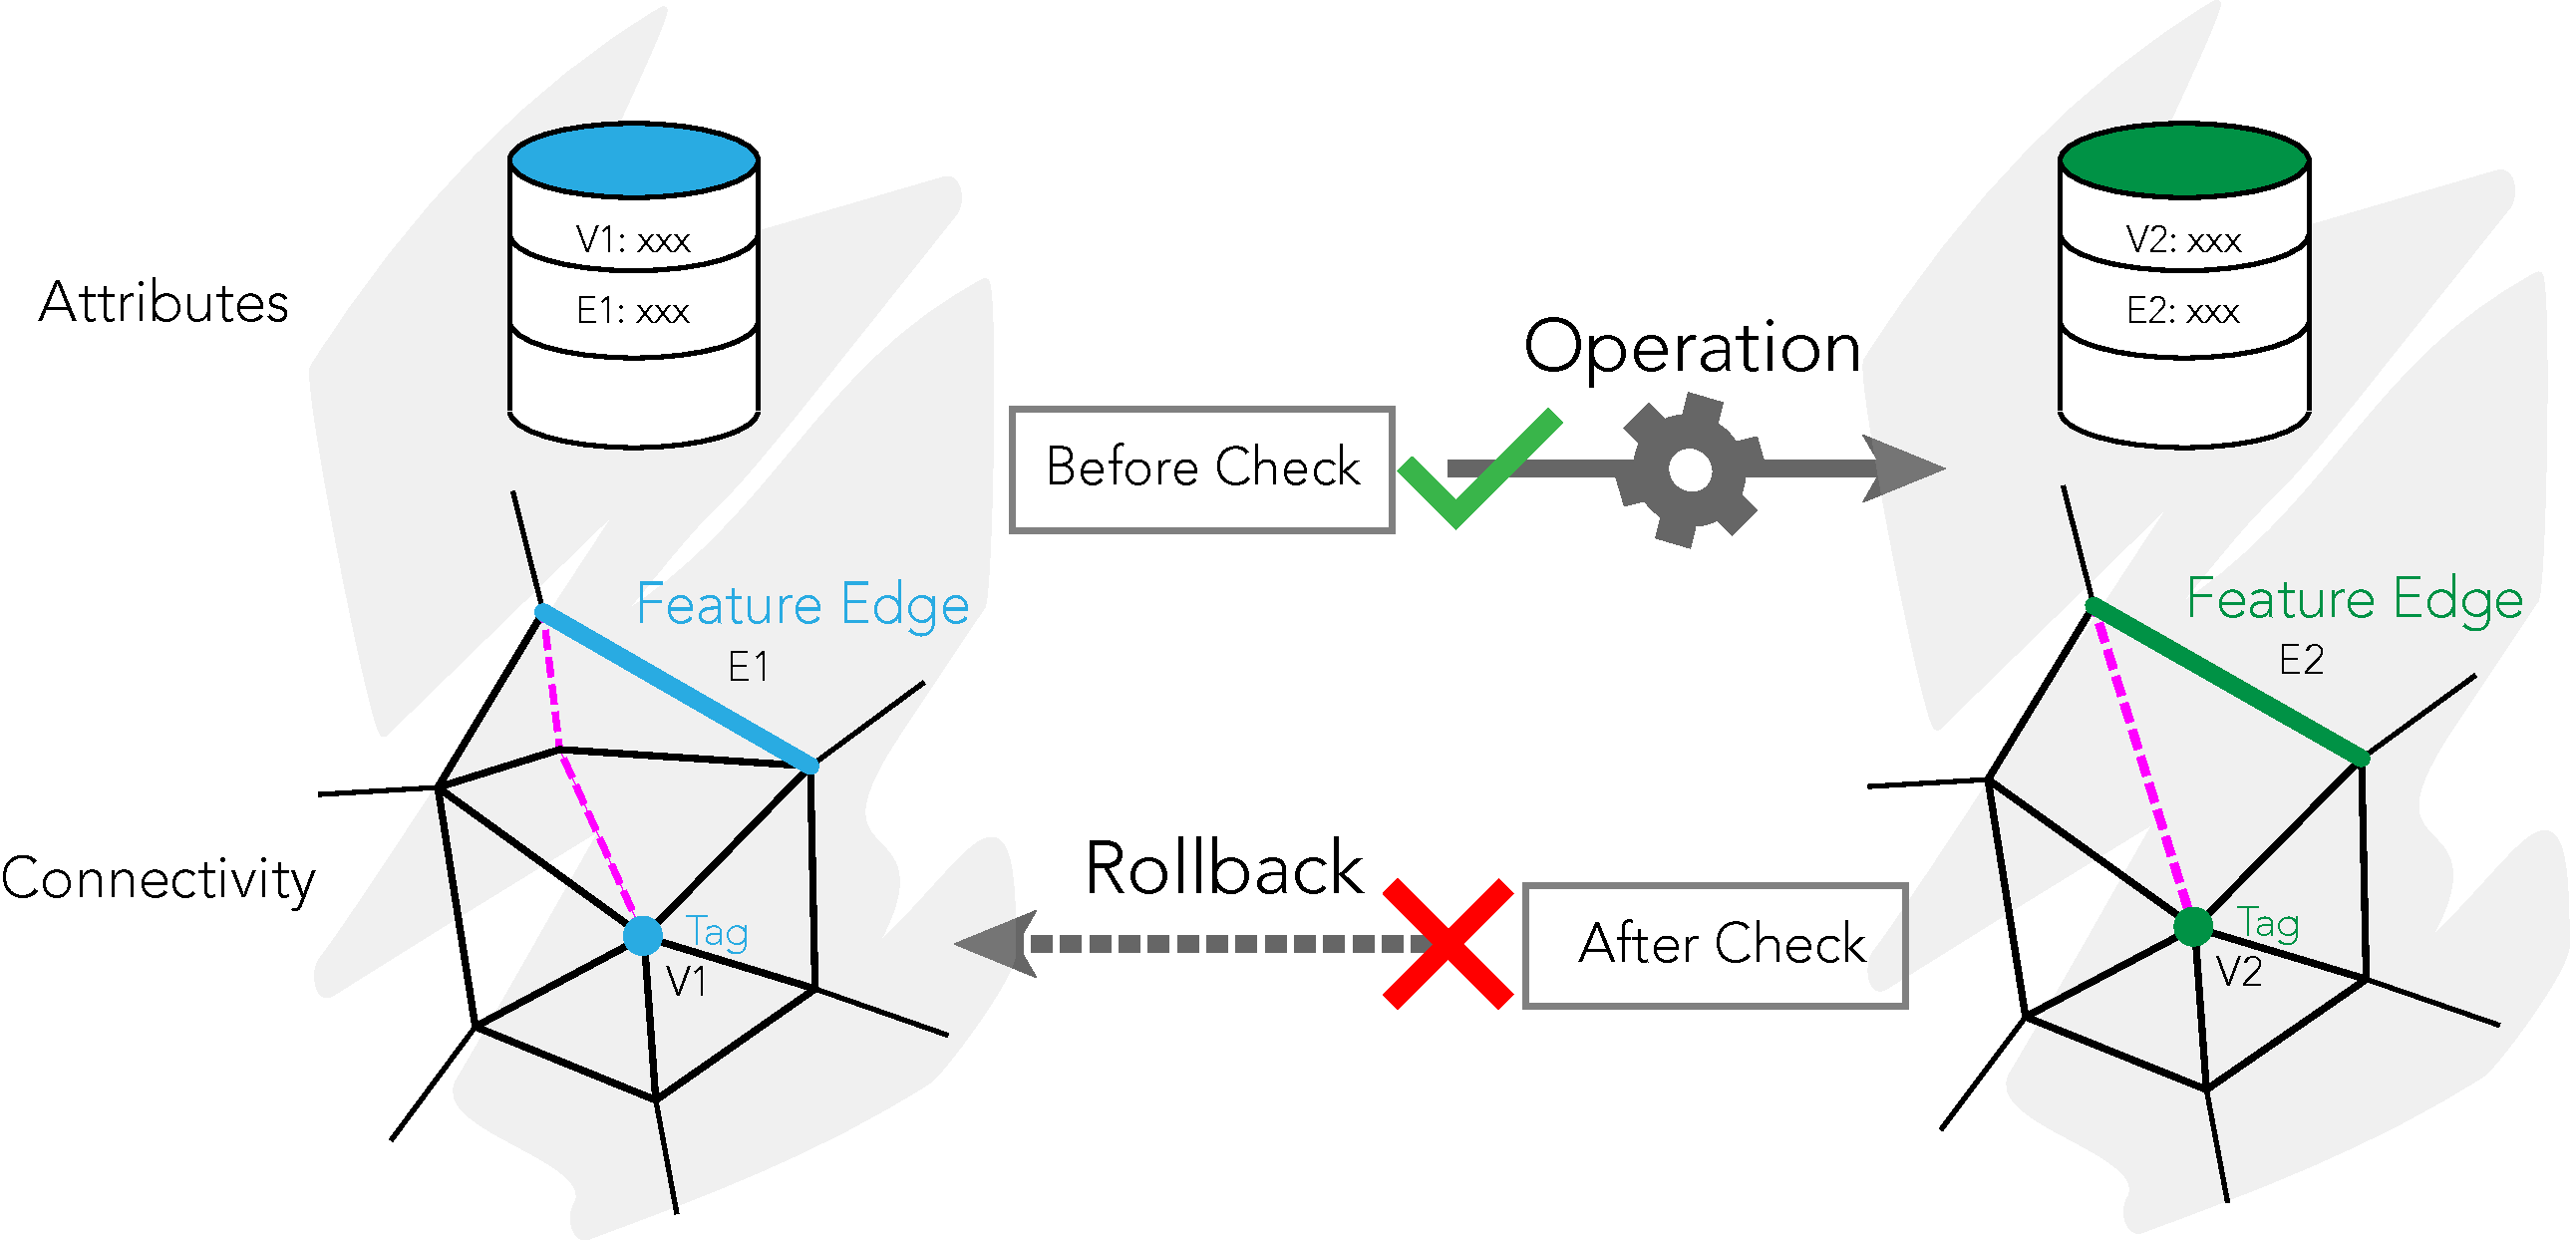
\includegraphics[width=\linewidth]{wmtk-tex/figs/pipeline_illustration.pdf}
    \caption{{Overview of the components behind our specification. A mesh is represented trough its topology, implemented by our library, and a list of user provided attributes. Before an operation is attempted, we explicitly perform a pre-check, and, if successful, we generate a mesh (attributes and topology). At this point, we trigger the after check to validate the operation (e.g., check if the newly generate mesh has positive volume). In case the after check fails, we \emph{automatically} rollback the operation and restore the mesh to its previous \emph{valid} state.}}
    \label{fig:pipeline}
\end{figure}

\section{Method}

Our declarative specification is designed to remove the burden of low-level management of the mesh connectivity {and attributes}, allowing an algorithm designer to focus only on high-level requirements. The design consists of five components. 

\subsection{{Mesh editing components}}

\paragraph{Operation Rollback.}
It is common to perform mesh editing to improve a given energy functional, such as mesh quality or element size. However, due to the discrete nature of the operations, it is not possible to use standard smooth optimization techniques, and instead the effect of the energy is evaluated before and after every operation to measure its effect on the energy. This is commonly implemented using an ad-hoc energy evaluation that ``simulates'' the operation only for the purpose of measuring the energy change. This simulation is complex (especially in 3D), and error-prone, as not only the connectivity changes, but the energy likely depends on properties attached to mesh elements, which needs to be updated accordingly.

We propose instead to make this process {opaque} to the user, providing to the user-code an explicit copy of the  mesh (and up to date attributes) \emph{before and after} the operation is performed to allow an easy and reliable energy evaluation. The correctness and efficiency of this process is handled by the runtime. This reduces the complexity of mesh editing considerably in our experience, as it makes them more similar to traditional finite difference approaches where the energy is evaluated on different points on the domain to approximate its derivative.

\paragraph{Explicit Invariants.}
It is common to have a set of desiderata on the mesh that needs to be satisfied, such as avoiding triangle insertions or self-intersections. Given the complexity of a mesh editing algorithm it is difficult to ensure that they are satisfied, as these conditions needs to be checked after every operation is applied (and they often depend on attributes too, such as vertex positions).

We propose to make these invariants explicit, and delegate to the library the task of ensuring that they are checked after every mesh modifications, and after the input is loaded. In this way, not only the code is simpler, but it is much easier to ensure correctness, as the checks are handled transparently by the library.

\paragraph{Explicit Attribute Update.}
Mesh attributes are usually handled by low-level meshing libraries, allowing to attach them to the desired mesh element (vertex, edge, face, triangle, or tetrahedra). However, the handling of attributes after a local operation is performed is usually a responsibility of the user code, as it is dependent on the application. 

We propose to make this process more explicit, requiring the user to provide the rules on how to update attributes after operation in a high-level specifications, and delegating the actual update to the library. This makes the specification more direct and less error-prone, and allows users to write algorithms without having to know the low-level details on how the local mesh operations work.

\paragraph{Parallel Scheduling.}
The type and scheduling of local operations is crucial in mesh editing algorithms. It usually involves maintaining a priority queue of operations, which is updated after every local operation.

We provide a direct way of controlling the operations performed and how the queue is updated. In the library, we can then distribute the work automatically on multiple threads, hiding from the user code the complexity of performing mesh editing operations in parallel and ensuring that race conditions are avoided. 

\paragraph{Abstract Mesh Navigation.}
Both invariant and attribute updates require navigating a mesh. Instead of relying on data-structure specific navigation, we favor the use of the cell tuple abstraction \cite{Brisson1989}. This allows the specification to be independent of the mesh data structure used in the library. The \texttt{Tuple} stores four indices  (three for surface meshes), vertex, edge, face, and tetrahedron and provides a single function per index, called \texttt{switch}, to change one index while keeping the other indices fixed. For instance \texttt{switch\_vertex} changes the vertex index while keeping edge, face, and tetrahedron fixed which has the effect of selecting the opposite vertex on an edge.

%%%%%%%%%%%%%%%%%%%%%%%%%%%%%%%%%%%%%%%%%%%%%%%%%%%%%%%%%
\subsection{Declarative Specification}

%As aforementioned explained, the key idea of our declarative specification is to decouple the low-level implementation details from the logic of the actual algorithm. 
%The key idea is to provide an high-level API hiding the complexity for topology changes, and delegate to the application code the update of vertex, edge, face, and tetrahedron attributes. For instance, our meshes do not store any geometric information such as vertex positions. 

Our API provides two abstractions: a \texttt{TetMesh} (and \texttt{TriMesh} class for 2D) (Algorithm \ref{algo:tetmesh}), and a \texttt{Scheduler} (Algorithm~\ref{algo:scheduler}).

\begin{longlisting}
\inputminted{cpp}{wmtk-tex/code/tetmesh.cpp}
\caption{API of our \texttt{TetMesh} class.}
\label{algo:tetmesh}
\end{longlisting}

% \begin{algorithm}
% \inputminted{cpp}{wmtk-tex/code/trimesh.cpp}
% \caption{API of our \texttt{TriMesh} class.}
% \label{algo:trimesh}
% \end{algorithm}


\begin{longlisting}
\inputminted{cpp}{wmtk-tex/code/scheduler.cpp}
\caption{API of our \texttt{Scheduler}.}
\label{algo:scheduler}
\end{longlisting}

\paragraph{Mesh Classes}
Both the \texttt{TetMesh} and \texttt{TriMesh} classes provide the basic local operations (e.g., edge split or collapse) and, for each operation, their corresponding \emph{before} and \emph{after} methods. The mesh class is responsible of implementing the operations changing the topology, and the application code must \emph{only} override the before and after methods to update attributes. The before method has a view of the mesh before the operation, and can thus navigate it to cache local attributes, while the after method has a view after the operation is performed, and it is responsible for updating attributes. In the simple case of regular subdivision of a triangle mesh, the \texttt{split\_before} caches the coordinates of the two edge endpoints, and the \texttt{split\_after} computes the position of the newly inserted vertex by averaging them. 

In addition, the mesh class provides a method, which can be overridden by the user code, that \emph{automatically} verifies user-provided invariants (e.g., maintain positive elements' volume). All user-provided methods return a Boolean status to notify the mesh classes if the operation fails; in case it does, our API rolls back the operation and restores the topology to the previous valid state. As the connectivity and attributes management is handled by the class, this ensures that, in case of failure of the operation, the mesh will go back to a valid state.

Our API provides the standard local operations: edge collapsing. edge/face swapping, edge splitting, and smoothing. We also provide an additional, non standard, operation: triangle insertion. This operation is an enhanced version of splitting where multiple edges, faces, and tetrahedra are subdivided to represent an input  triangle provided as input. This operation is useful to compute mesh arrangements, and it is also used in meshing algorithms \cite{Hu:2019:fTetWild}.

Since the \texttt{TetMesh} class only handles topology, the operation requires the list of edges and tetrahedron the input triangle intersects. Internally it subdivides all of them, and generates a valid tetrahedral mesh using the connectivity table in~\cite{Hu:2019:fTetWild}. The before operation provides the user the list of  faces that will be changed by the operation, allowing the user code to explore the mesh and cache attributes,  while the after provides a mapping between the old faces and any newly inserted face in the mesh.


\paragraph{Scheduler}
The second part of our API is the \texttt{Scheduler} that is responsible to control the order of the individual operations and then execute a list of operations. The main purpose of the scheduler is to abstract the operation order and hide parallelization details from the user. Our scheduler provides customizable callbacks, including,
\begin{itemize}
    \item \emph{Priority} to order the local mesh edit operations.
    \item \emph{Renew neighbor tuples} that is invoked after a successful operation, to add newly created tuples and operations into the queue.
    \item \emph{Lock vertices} that provides information on the affected region for the operation, and avoiding conflicts.
    \item \emph{Stopping criterion} that is checked periodically to terminate the program if certain criterion is met. For example, number of vertices, or quality criterion.
\end{itemize}




% \paragraph{Harmonic Tetrahedralization}
% \TODO{write me}


\subsection{Implementation.}

We implement a runtime for our specification in C++, using Intel oneTBB for parallelization.

\paragraph{Data Structure.} We opt for an indexed data structure, where we explicitly represent the vertices and the simplex of higher dimension (triangle for 2D, tetrahedra for 3D). Each vertex explicitly stores a list of incident simplices, and each simplex stores a sorted list of its vertices. While not the most efficient option for navigation, this data structure makes the implementation of local operation much simpler. 

\paragraph{Parallelization.} To avoid conflicts between local operations working on the same part of the mesh, we introduce a synchronization mechanism using locks. 

\begin{figure}\centering\footnotesize
    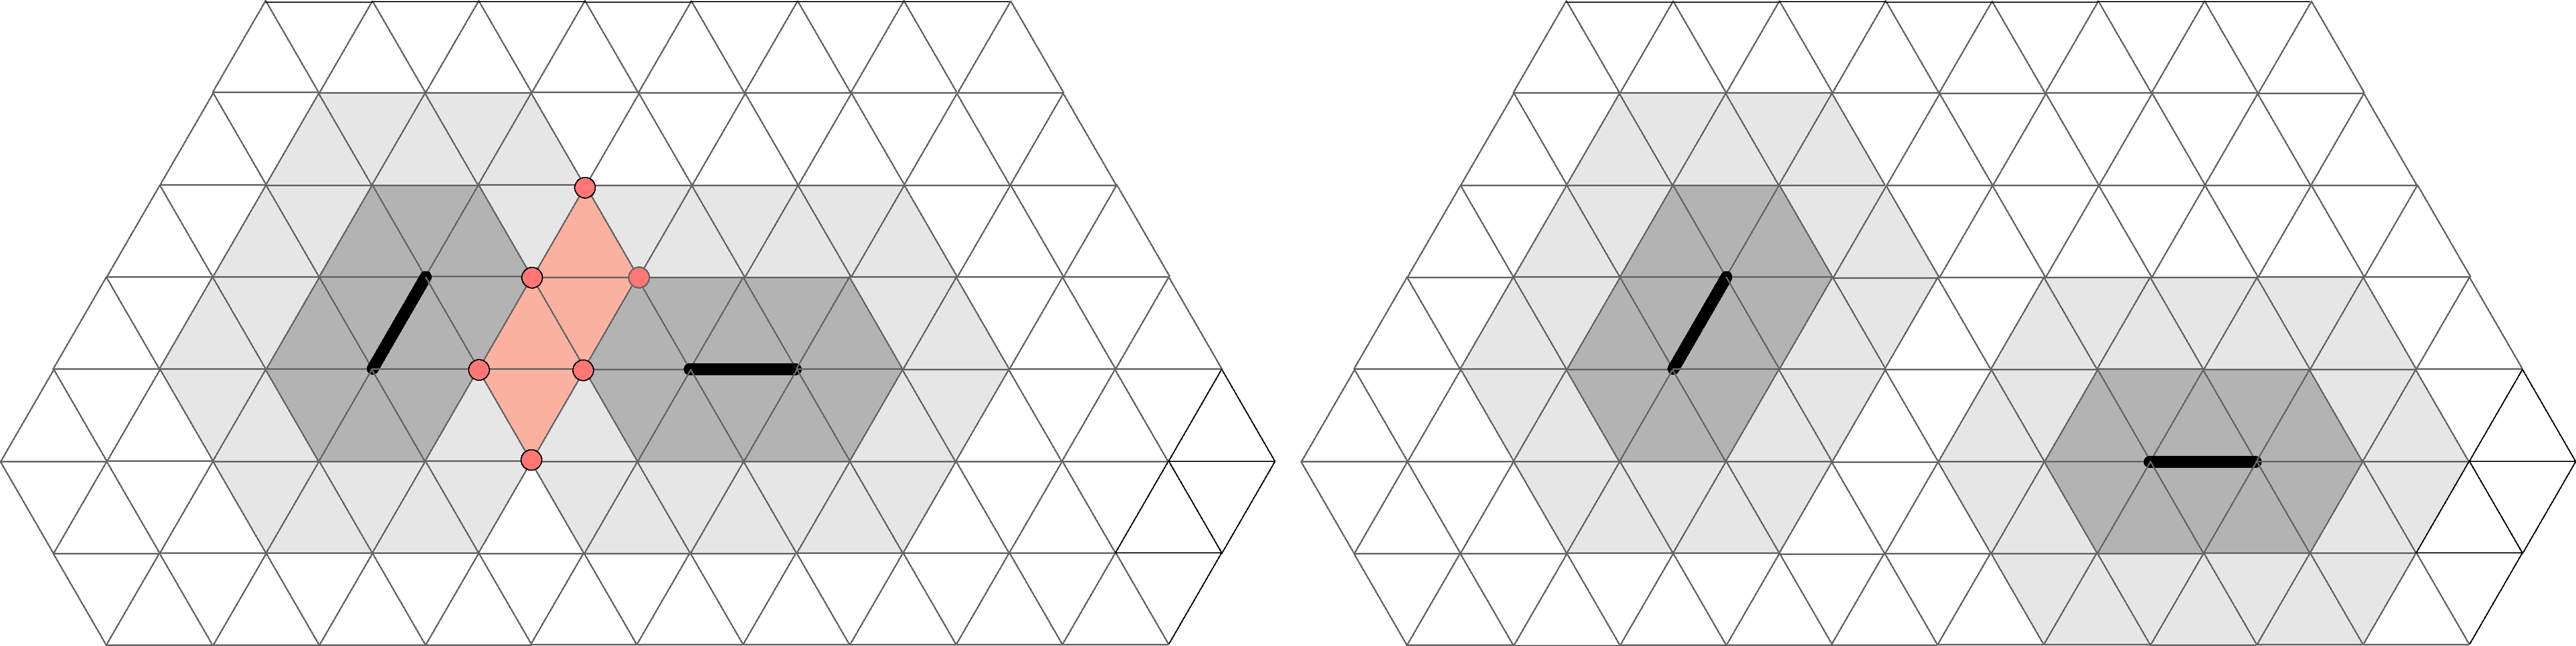
\includegraphics[width=\linewidth]{wmtk-tex/figs/lock_illustration}
    \caption{{Example of the locking region for two edges. In the example the operation requires locking a two-ring neighborhood (e.g.,  for the edge collapse operation). If the two edges are sufficiently far (right) both operations can be safely executed in parallel. When the two edges are close (left) the operations might fail acquiring the mutexes in the shared area.}}
    \label{fig:lock-example}
\end{figure}

Each mesh vertex is associated with a mutex. Whenever a thread wants to access (read/write) any attribute stored in a vertex, edge, triangle, or tetrahedron it must first acquire a lock on \emph{all} the vertices of the tetrahedron containing the element(s) storing the attribute (Figure~\ref{fig:lock-example}). For example, if a thread wants to read a value on an edge of a 3D mesh, it first needs to acquire a lock on all vertices of all the tetrahedra containing that edge. This mechanism is used also for mesh navigation, and for updating the mesh connectivity. 

At a first look, this mechanism might seem cumbersome and expensive. However, we rely on asynchronous, tentative lock acquisition operations. We \emph{try} to acquire the lock, and give up if the lock is already taken by another thread. These operations are efficient on modern hardware and dramatically improve the performance, while avoiding deadlocks. A downside is that an operation might be skipped due to impossibility of acquiring a mutex. These operations are retried for several times (by default 10 times) and run serially if the still do not succeed. Before performing any local operation, we try to acquire the lock on vertices in the 1-ring or 2-ring of the vertex involved in the operation. For example, a vertex smoothing operation requires acquiring the 1-ring vertex neighborhood of the smoothed vertex, while an edge-collapse operation on an edge $(v_1, v_2)$ requires acquiring the lock on the 2-ring vertex neighborhood of both $v_1$ and $v_2$
({Figure ~\ref{fig:lock-example}}).

Finally, since we partition the input mesh using {Morton Encoding} \cite{karras2012maximizing}, the amount of conflicts (and skipped operations) is low.



\subsection{{Example: Shortest Edge Collapse}}

We show how the library is used in a classical example, shortest edge collapse. In this case, we add a 3D position to every vertex as a vertex attribute (by default, there are no attributes attached to mesh elements). For every attribute and for every operation we plan to use in the scheduler, we need to provide a function that updates such attribute (Algorithm~\ref{algo:shortest}). In the \texttt{collapse\_before} function, we cache the two vertex coordinates associated with the collapsed edge represented by \texttt{Tuple t}. In the \texttt{collapse\_after} function, we generate a new vertex in the middle of the two endpoints of the collapsed edge. %For instance, this method can be changed to collapse to \texttt{v1p} by simply assigning \texttt{p} to \texttt{v1p}.

\begin{longlisting}
\inputminted{cpp}{wmtk-tex/code/shortest.cpp}
\caption{Overridden methods in \texttt{TriMesh} sub-class to implement shortest edge collapse.}
\label{algo:shortest}
\end{longlisting}

Equipped with the 3D position attribute, which at this point will be automatically kept up to date by the library, we can now schedule the collapse operation (Algorithm \ref{algo:shortest-sced}). For shortest edge collapse, we want to attempt to collapse all edges, prioritizing the shortest ones, until we reach a fixed number of collapses \texttt{n\_collapse}: in the code we registering the operation type (\texttt{ops}), specify how to update the queue after an operation (\texttt{renew}) by adding all the neighbouring edges, and specifying the edge length as a priority (\texttt{priority}). Note that the {outdated} elements in the queue that are affected by a local operation are automatically invalidated using a tagging mechanism on the tuples which is opaque to the user.

% TODO code too long 
\begin{longlisting}
\inputminted{cpp}{wmtk-tex/code/shortest-sched.cpp}
\caption{Scheduler setup for the schedule shortest edge collapse.}
\label{algo:shortest-sced}
\end{longlisting}
\section{Applications}
\label{wmtk:sec:applications}

To showcase the generality and effectiveness of our approach, we implement five popular mesh editing algorithms in our framework, and compare them with reference implementations. Overall, the performance of our method are competitive for surface applications, but the overhead due to the approach generality is higher in 3D, leading to higher running time.

\paragraph{Shortest Edge Collapsing}

The simplest algorithm for simplifying a triangle edge is shortest edge collapse \cite{hoppe1996progressive}, which performs a series of collapse operations prioritizing the shorter edges. The algorithm requires only one local operation, edge collapse. A common criteria for termination is reaching a desired number of mesh elements. We compare our implementation with the ``decimate'' implementation in libigl \cite{jacobson2016libigl}. The serial libigl implementation is comparable when running the algorithms serially, and our parallel implementation is up to 9 times faster when using 32 threads (Figure \ref{fig:decimate}).

\begin{figure}
    \centering\footnotesize
    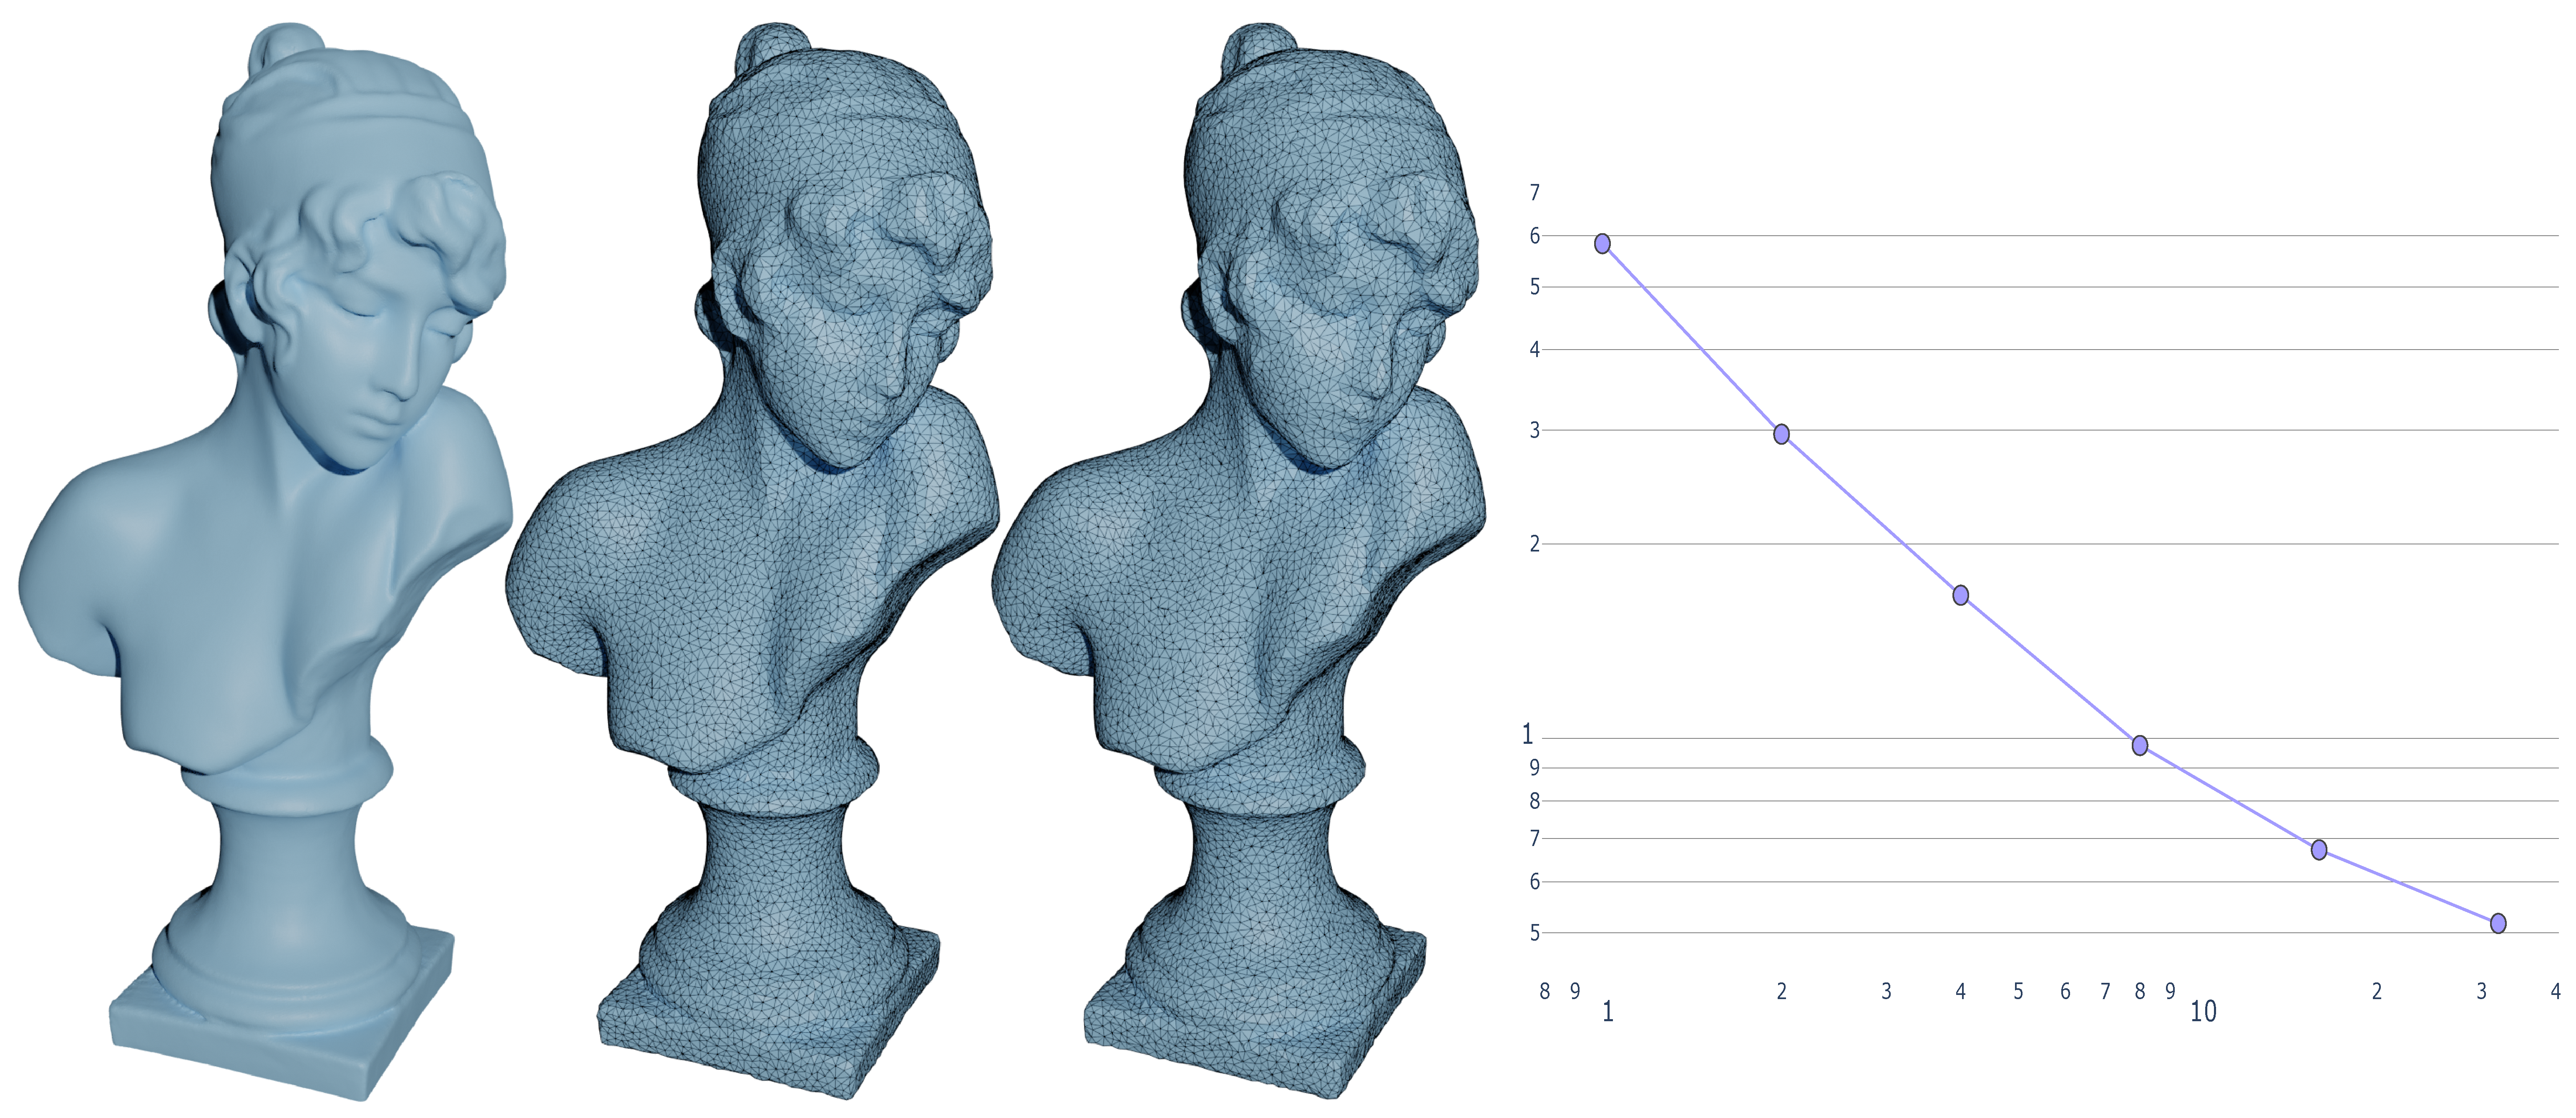
\includegraphics[width=\linewidth]{wmtk-tex/figs/2d-sec-statue.pdf}
    \parbox{.15\linewidth}{\centering Input}\hfill
    \parbox{.15\linewidth}{\centering libigl}
    \hfill
    \parbox{.15\linewidth}{\centering Output}\hfill
    \parbox{.3\linewidth}{\centering Timing}\par
    \caption{
    Comparison of our parallel implementation (32 threads) of shortest edge collapse (scalability plot on the right, from 1 to 32 threads) of a model with $281,724$ faces with the serial version in libigl. {Both libigl and our output have $28,168$ faces and comparable edge length (1.058 for libigl versus 1.061 for ours). Our serial method runs in 4.9s (5.84s on a single thread, 0.52s with 32 thread, leading to a speedup of $11\times$), while libigl runs in 2.74s.}}
    
    % 0 thread: 4.9s
    % 1 thread: 5.84s
    % 2 thread: 2.96s
    % 4 thread: 1.67s
    % 8 thread: 0.98s
    % 16 thread: 0.67s
    % 32 thread: 0.52s
    \label{fig:decimate}
\end{figure}

\paragraph{QSlim}
{We use our framework to implement QSlim~\cite{garland1997surface}. 
QSlim collapse edges based on the planarity of the two adjacent faces measured with an error quadric. The algorithm continues to collapse until it reaches a target number of edges. We compare our implementation with the QSlim implementation in libigl \cite{jacobson2016libigl}. The serial libigl implementation is 8 times faster than our implementation, due to their direct manipulations of elements in the queue with each collapse. But our parallel implementation is twice as fast when using 16 threads (Figure \ref{fig:qslim})}.

\begin{figure}
    \centering\footnotesize
    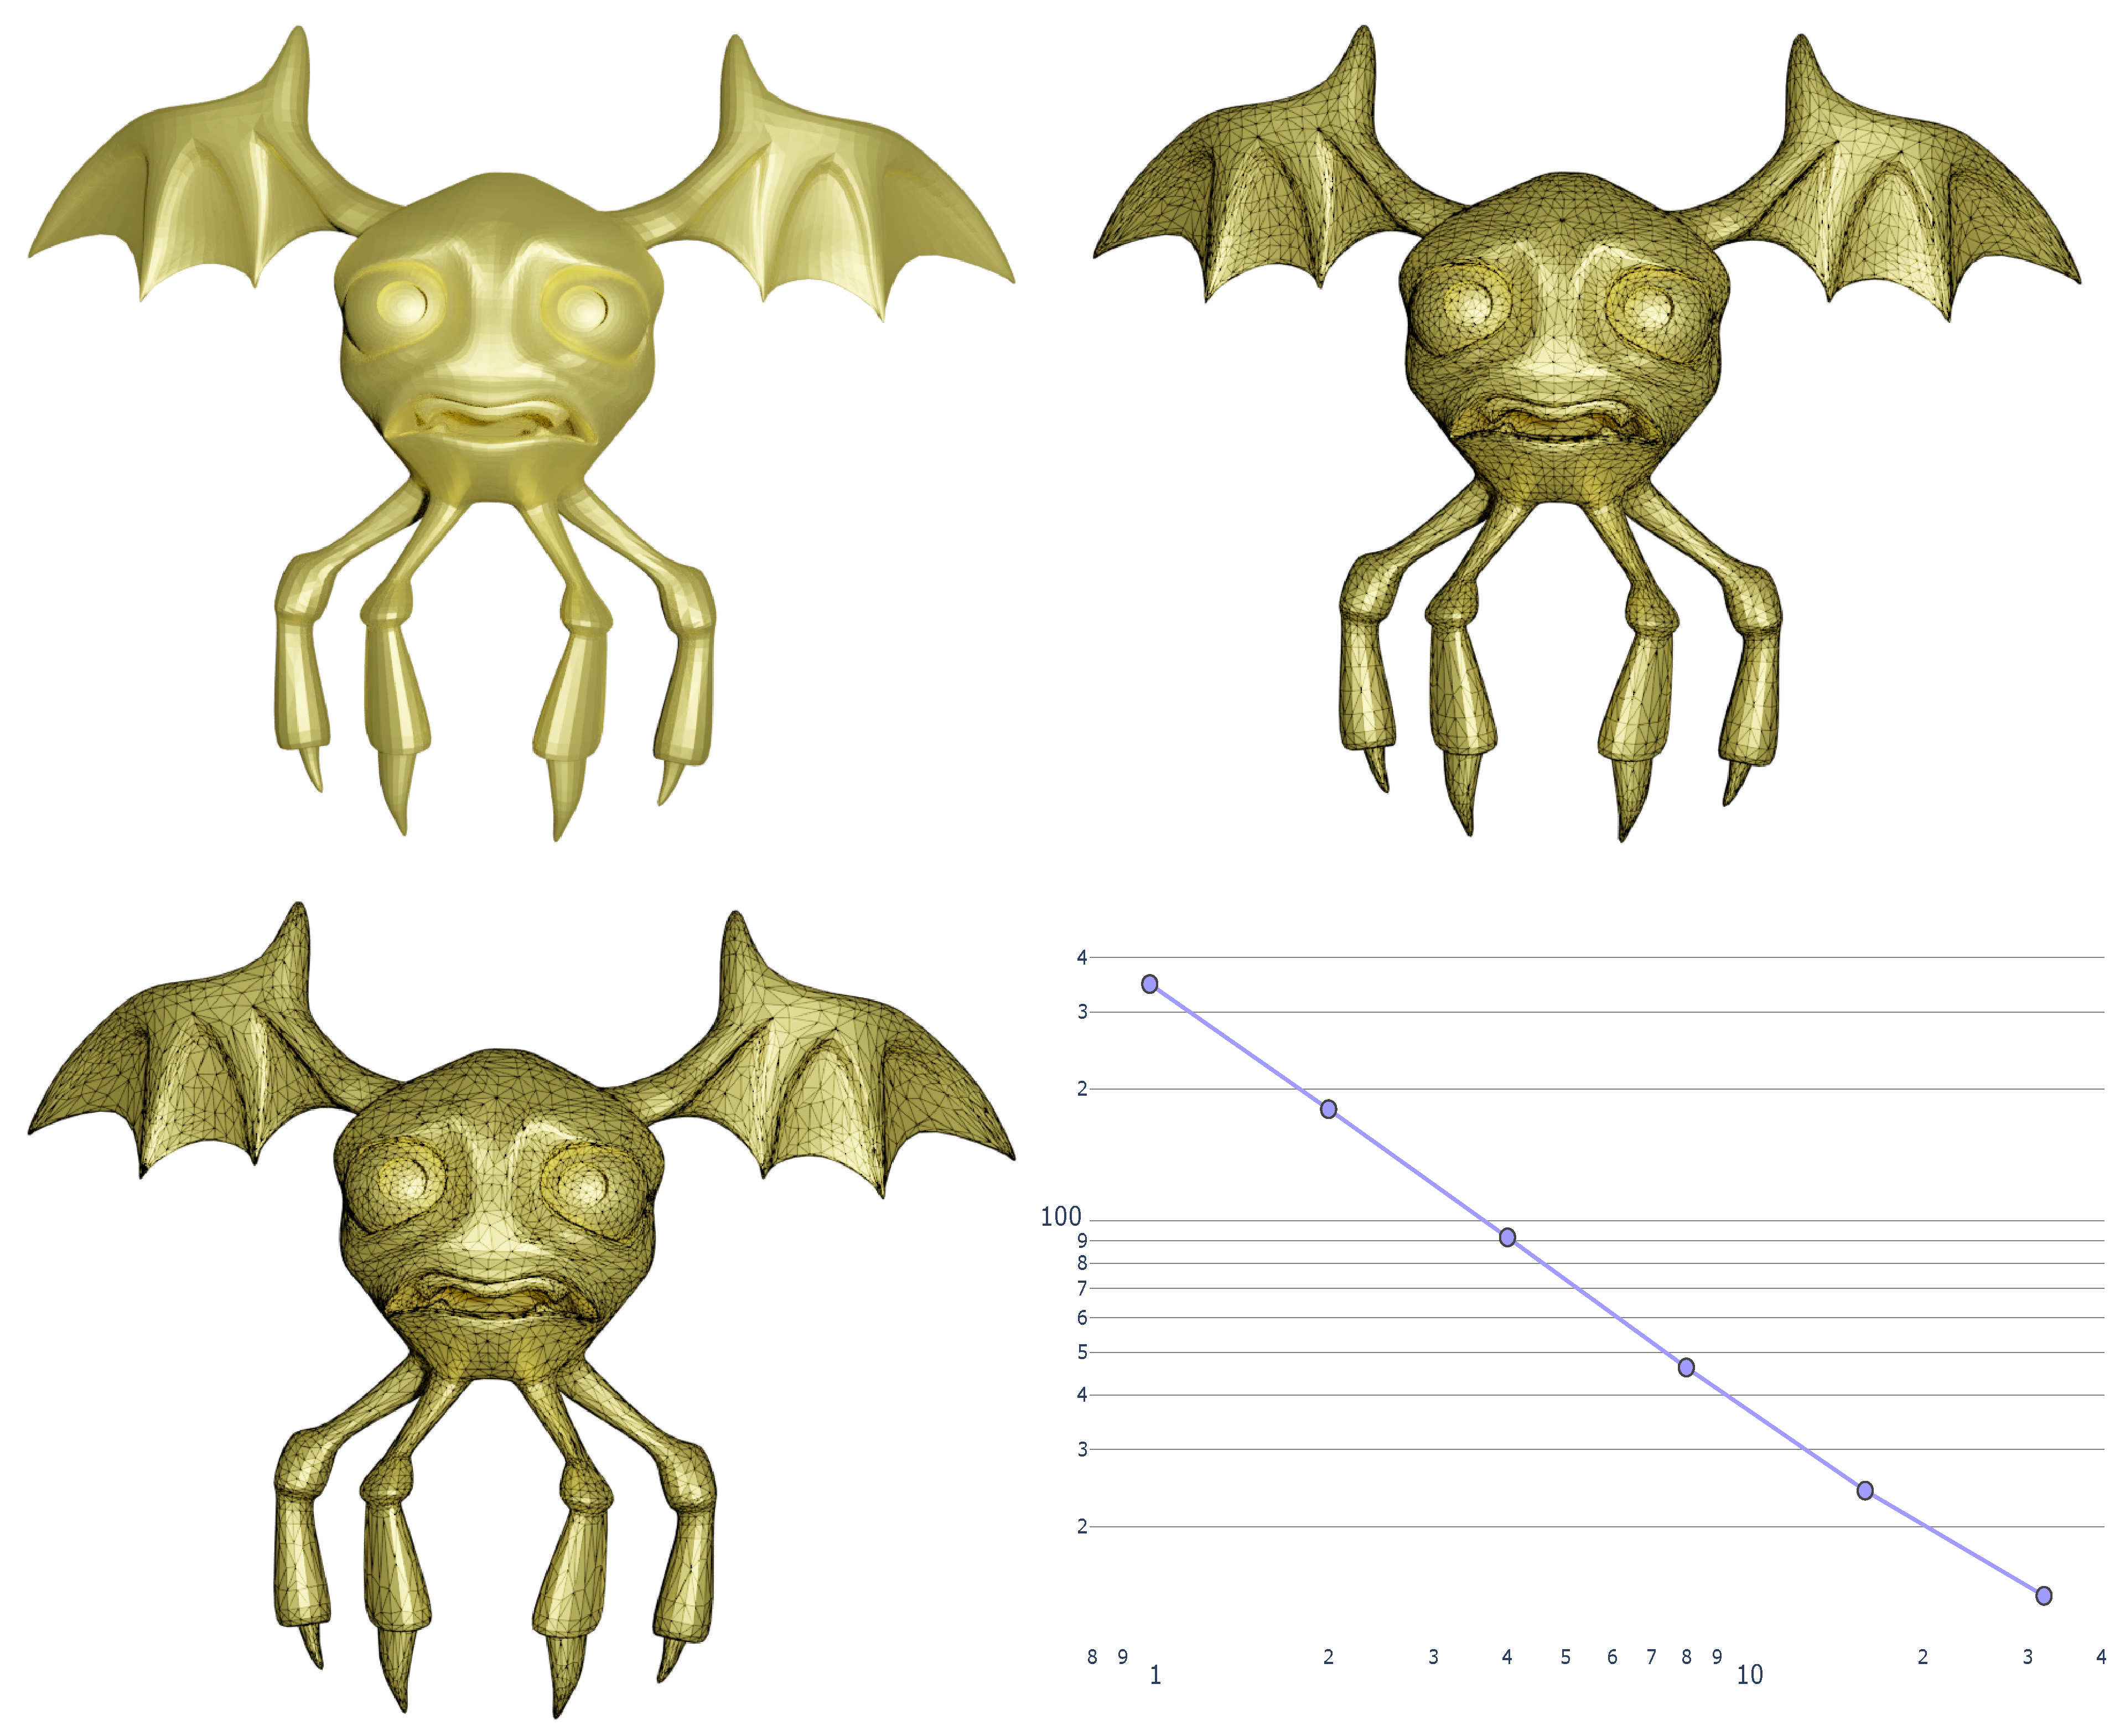
\includegraphics[width=\linewidth]{wmtk-tex/figs/2d-qslim.pdf}
    \caption{{Comparison of our parallel implementation of QSlim with the serial version in libigl for a model with $1,909,755$ faces. Top right, the libigl output has $17,891$ faces and takes 41.26s. Bottom left, our output has $17,906$ faces and runs in 306.59s.  Our implementation scales well: 347.59s with one thread and 13.88s with 32 (25$\times$ speedup).}
    }
    \label{fig:qslim}
\end{figure}

    % 0 thread: 306.59s
    % 1 thread: 347.59s
    % 2 thread: 179.84s
    % 4 thread: 91.62s
    % 8 thread: 46.19s
    % 16 thread: 24.16s
    % 32 thread: 13.88s

\paragraph{Isotropic Remeshing}

We implemented the {widely used} algorithm for isotropic remeshing proposed in \cite{botsch2004remeshing}. This algorithm alternates edge collapse, edge flips, edge splits, and tangential smoothing to obtain a mesh that is isotropic (i.e. all elements have the same size) and where all triangles are close to equilateral. The process is guided by a user-provided target edge length $L$, and terminates when no local operation leads to either an improvement in the desired edge lengths or an improvement in vertex valence \cite{botsch2004remeshing}.

In Figure~\ref{fig:uniform}, we compare our implementation of \cite{botsch2004remeshing} with the implementation in OpenFlipper~\cite{mobius2010openflipper}.
The OpenFlipper implementation is 2.5 times faster when running on a single thread, and our implementation becomes faster after 4 threads are used (Figure \ref{fig:uniform}).

\begin{figure}
    \centering\footnotesize
    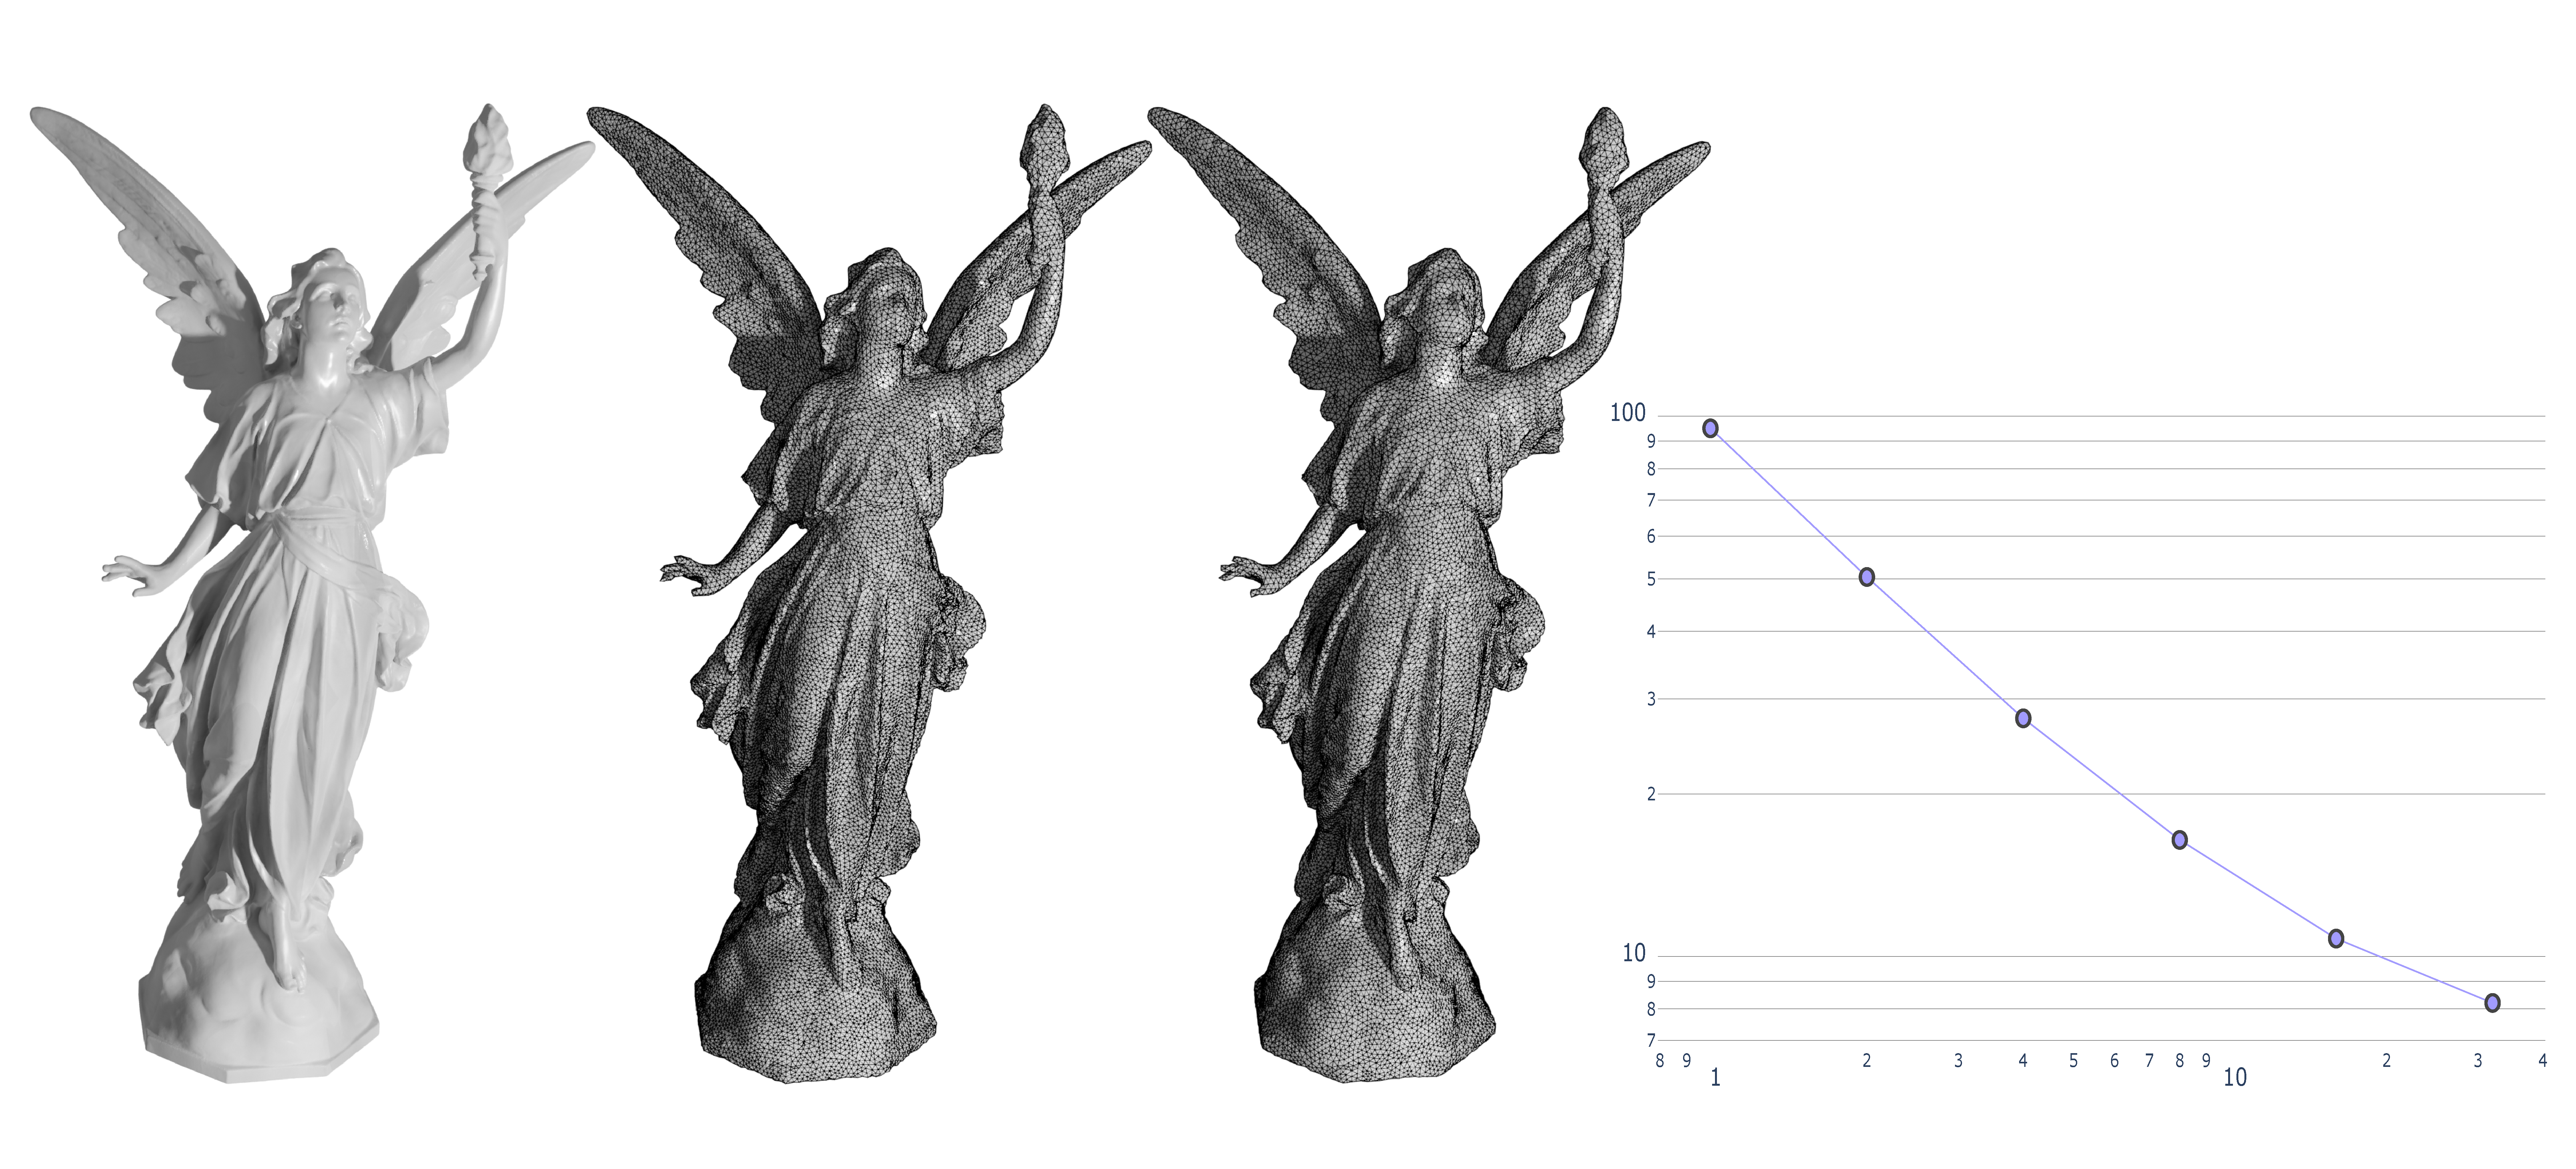
\includegraphics[width=\linewidth]{wmtk-tex/figs/2d-remeshing-lucy.pdf}
    \caption{Example of uniform remeshing a model with $2,529,744$ triangles (left) with the same target edge length. Middle, \cite{mobius2010openflipper} remeshes it to $78,322$ faces in 31.96 seconds. On the right is our
    32-thread implementation, which generates $71,640$ triangles in 8.2 seconds (78.34s serial, 95.0s for a single thread, leading to a speedup of 11$\times$). The difference in density of the meshes is due to differences in the detail of the implementation, which makes the two methods reach an average vertex valence of 5.999, and a similar target edge length (differ 0.01\% of the bounding box diagonal length) with a different element budget.}
    \label{fig:uniform}
    % wmtk avg length 8.86, opf: 8.59, BB 1922.46
    % openfliiper 31.96s
    
    % 0 thread: 78.34s
    % 1 thread: 95.0s
    % 2 thread: 50.42s
    % 4 thread: 27.6s
    % 8 thread: 16.44s
    % 16 thread: 10.8s
    % 32 thread: 8.2s
    
\end{figure}

\paragraph{Harmonic Triangulations}

The \emph{harmonic triangulations} algorithm has been introduced as an alternative to sliver exudation in the Delaunay tetrahedralization pipeline to efficiently reduce sliver tetrahedra. The original paper \cite{Alexa:2019} proposes to use both flip and smoothing operations. 

The code provided by the authors implements a reduced version of the algorithm proposed in the paper, restricting the optimization to 3-2 edge swap operations. We thus implemented both a reduced version for a fair comparison (Figure \ref{fig:harmonic}) and a complete version. Our more generic framework is twice as slower than the hand-optimized code written by the authors when running serially, and it is 2 times faster when running on 32 threads (Figure \ref{fig:harmonic}).

% Reference: 
% Total time for harmonizing Delaunay triangulation: 6.37256 seconds
\begin{figure}
    \centering\footnotesize
    \includegraphics[width=\linewidth]{wmtk-tex/figs/3d-harmonic-gauss.pdf}
    % \parbox{.2\linewidth}{\centering Input\\\#V = 1 million}\hfill
    \parbox{.2\linewidth}{\centering Reference}\hfill
    % \\\#T =6MM,  6.37 s\\Mean Harmonic Index 0.547}\hfill % 5.25 on Kirby, 6.38 on sonic
    \parbox{.2\linewidth}{\centering Output}\hfill
    % \\\#T = 6MM, 3.82 s (32 threads) \\Mean Harmonic Index 0.554}\hfill
    \parbox{.3\linewidth}{\centering Timing}\par
    \caption{Example of \emph{Harmonic Triangulations} starting with one million Gaussian distributed random points. {Both our and the reference implementation reach a similar target number of tetrahedra (5.9 million for the reference and 6.1 million for ours, due to a difference in operation ordering) and a similar Mean Harmonic Index (0.547 for the reference and 0.554 for ours). Our method takes 3.82s with 32 threads (15.49s serial, 40.49s on a single thread, speedup of 11$\times$), while the reference serial implementation takes 6.37s.}}
    \label{fig:harmonic}
    
    % harmonic: 
    
    % 0 thread: 15.49s
    % 1 thread: 40.49s
    % 2 thread: 21.6s
    % 4 thread: 12.3s
    % 8 thread: 7.27s
    % 16 thread: 4.99s
    % 32 thread: 3.82s
    
\end{figure}

\paragraph{Tetrahedral Meshing}

The TetWild algorithm is a tetrahedral meshing algorithm with minimal input requirements: given an input triangle soup, it can generate a tetrahedral mesh which approximates its volume. We {take inspiration from} the original algorithm introduced in \cite{hu2018tetrahedral,Hu:2019:fTetWild} with a few modifications: (1) we use the insertion operation \cite{Hu:2019:fTetWild} (using rational coordinates) as a replacement for their BSP partitioning, as this simplifies the implementation, (2) we use the envelope proposed in \cite{Wang:2020:FE} instead of sampling, and (3) we use 2-3 face swapping, 3-2 and 4-4 edge swapping operations, to simplify the implementation. We show results on two models in Figure \ref{fig:tetwild}: the results are very similar to the original implementation, and our version is 2 times faster when using 8 threads. {We experimentally observe that our framework scales well up to 8 threads, after that the algorithm becomes slower. This is because, as we increase the number of threads and partitions, the frequent conflict in tetrahedral mesh edge operations affects the parallel performance. We believe that this observation might be useful for the future design of high performance concurrent mesh generation algorithms.}
% faster now!
% latest.  original: 287.577s


% 0 thread: 452.42s
    % 1 thread: 521.47s
    % 2 thread: 300.48s
    % 4 thread: 197.68s
    % 8 thread: 153.33s
    % 16 thread: 176.82s
    % 32 thread: 207.35s
% 0.000000000000000000e+00,4.524295280000000048e+02
% 1.000000000000000000e+00,5.214727839999999333e+02
% 2.000000000000000000e+00,3.004886300000000006e+02
% 4.000000000000000000e+00,1.976867799999999988e+02
% 8.000000000000000000e+00,1.533386629999999968e+02
% 1.600000000000000000e+01,1.768291299999999922e+02
% 3.200000000000000000e+01,2.207351280000000031e+02


\begin{figure}
    \centering\footnotesize
    \includegraphics[width=\linewidth]{wmtk-tex/figs/3d-tetwild-dragon.pdf}
    \caption{Tetrahedralize a surface with $856,294$ faces. Original TetWild (top right) generates a mesh with $56,761$ tetrahedra in 287.58s; our reimplementation (bottom left) generates a mesh with $44,866$ tetrahedra in 153.33s with 8 threads (452.42s serial, 521.47s on a single thread, speedup of $3.4\times$). The difference in number of tetrahedra is likely due to the different order of scheduling of operations due to the partitioning.}
    \label{fig:tetwild}
\end{figure}

\subsection{Parallelization}
{
Enabling the parallelization mechanism introduces a minor slowdown as visible in the difference between the pure serial and one thread timings on our applications, due to the additional cost of allocating mutexes and to acquired them. The algorithm scales well in all 5 applications (figures \ref{fig:decimate}, \ref{fig:qslim}, \ref{fig:uniform}, \ref{fig:harmonic}, \ref{fig:tetwild}), obtaining a scaling speedup. 
%Our speedup is 11 \DP{check, 11 in both?} in triangular mesh applications with 32 threads and 11 \DP{11 gain?} in tetrahedral mesh applications using 32 threads. 
We would like to remark that thanks to our specification and our runtime, the serial and parallel implementation of the 5 algorithms above is almost identical.}

{An inevitable drawback of parallelization is that the algorithms cannot efficiently preserve ordering. For instance, in shortest edge collapse, every thread will try collapse edges in its own partition independently from the others. If one of these collapses append on the partition's interface, the thread will need to acquire a lock. In case of failure the collapse is postponed to a later stage thus not respecting the order (Figure~\ref{fig:limitation}). This is a rare event that is more problematic for fast operations.}


\begin{figure}\centering\footnotesize
    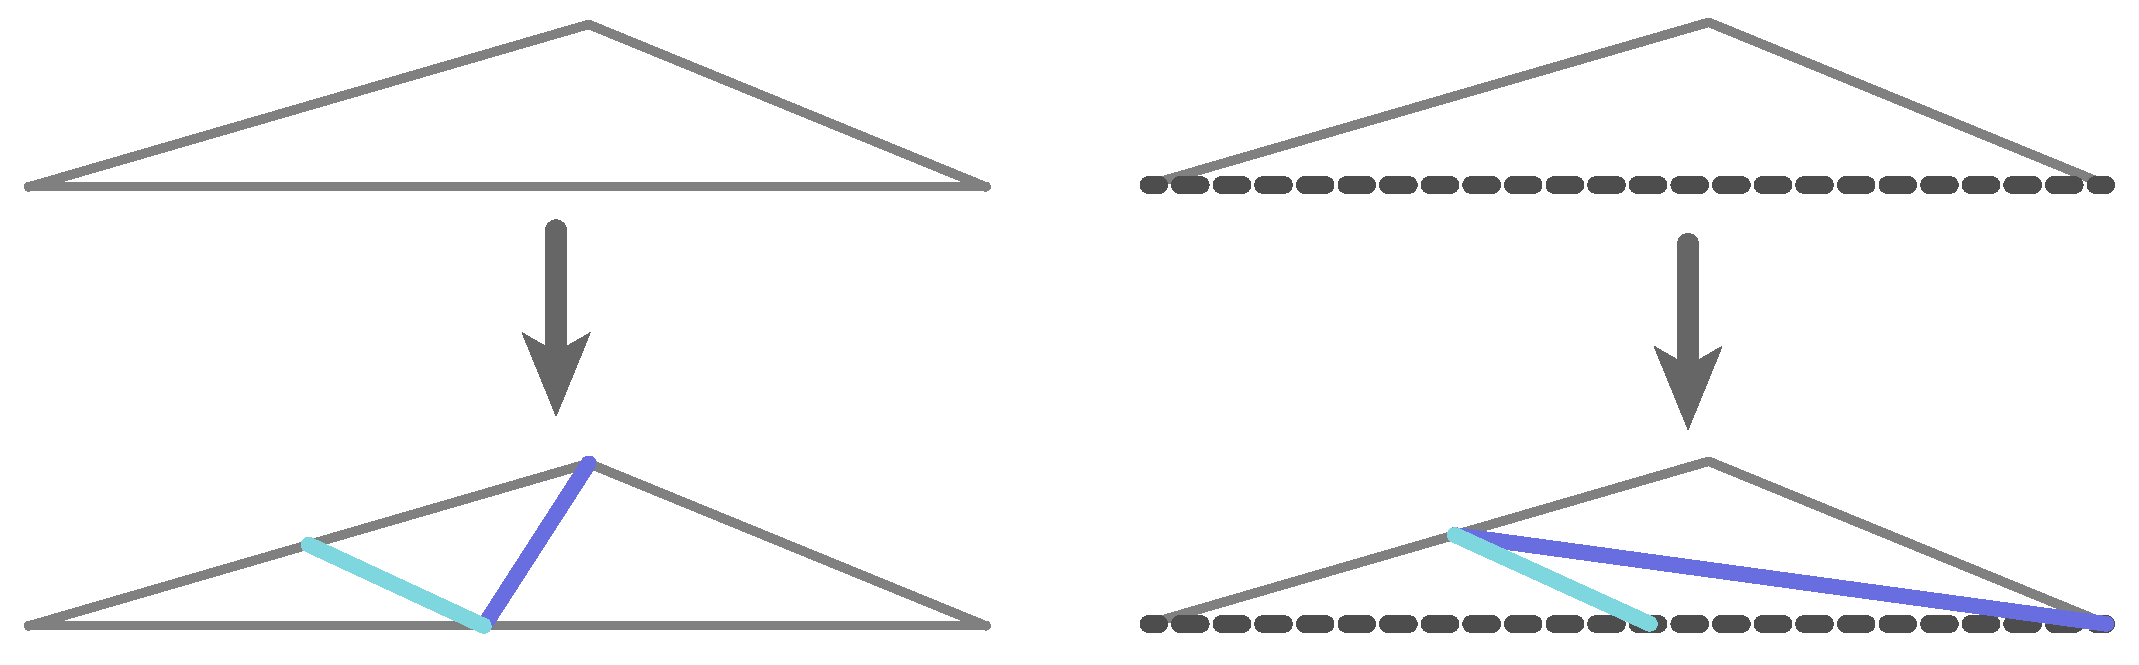
\includegraphics[width=\linewidth]{wmtk-tex/figs/limitation-of-para.pdf}
    \caption{{Example of splitting the longest edge on the bottom of the triangle. On the left, the edge can be split to generate the dark blue edge. In the next iteration, the left edge is split (by the light blue edge) leading to a decreasing maximum edge-length. On the left, the bottom edge is locked illustrated by a dashed line. In this case the next iteration splits the left edge (dark blue edge) and so on. As long as the dashed edge is locked it will never be split preventing the maximum edge length to decrease.}}
    \label{fig:limitation}
\end{figure}

\subsection{Algorithm Modifications}

A major motivation to invent and develop this declarative language is enabling easy customization of meshing algorithms. As an example, we add an additional termination criteria to the shortest edge collapse and uniform surface refinement.  Integrating the envelope check is straightforward with our approach, as it only requires adding the envelope check to the invariants. We use the open-source library proposed in \cite{Wang:2020:FE}, which allows to directly specify the maximal allowed surface deviation. The envelope adds a noticeable computational cost, which is ameliorated by our parallel implementation (figures \ref{fig:decimate_envelope} and \ref{fig:uniform_envelope}). 

\begin{figure}
    \centering\footnotesize
    \includegraphics[width=\linewidth]{wmtk-tex/figs/2d-sec-envelope.pdf}
    \parbox{.3\linewidth}{\centering Input}\hfill
    \parbox{.3\linewidth}{\centering Output}\hfill
    \parbox{.3\linewidth}{\centering Timing}\par
    \caption{Shortest edge collapse with envelope containment of a model with $857,976$ faces. {Our method successfully generates a mesh with $71,298$ faces in 37.49s with 32 threads (731.32s serial, 725.34s on a single thread, speedup of $20\times$).}}
    \label{fig:decimate_envelope}
    
    % 0 thread: 731.32s
    % 1 thread: 725.34s
    % 2 thread: 397.18s
    % 4 thread: 220.58s
    % 8 thread: 117.26s
    % 16 thread: 63.55s
    % 32 thread: 37.49s
    
\end{figure}


\begin{figure}
    \centering\footnotesize
    \includegraphics[width=\linewidth]{wmtk-tex/figs/2d-remeshing-headport-env.pdf}
    \parbox{.3\linewidth}{\centering Input}\hfill
    \parbox{.3\linewidth}{\centering Output}\hfill
    \parbox{.3\linewidth}{\centering Timing}\par
    \caption{Uniform remeshing with envelope containment check of a model with $198,918$ faces. {Our method produces a mesh with $68,202$ faces in 29.11s with 32 threads and 493.54s for a single thread (483.68s for the serial version) leading to a speedup of 16$\times$.}}
    \label{fig:uniform_envelope}
    
    % 0 thread: 483.68s
    % 1 thread: 493.54s
    % 2 thread: 258.88s
    % 4 thread: 139.36s
    % 8 thread: 77.38s
    % 16 thread: 43.16s
    % 32 thread: 29.11s

\end{figure}




\subsection{{Large-scale dataset validation}}

{To validate our framework we run our reimplementation of uniform remeshing and tetrahedral meshing on the Thingi10k dataset~\cite{zhou2016thingi10k}. We run all experiments serially on an individual node of an HPC cluster an Intel Xeon Platinum 8268 24C 205W 2.9GHz Processors limiting the runtime to 15 hours.}

{For uniform remeshing,  Figure~\ref{fig:2d-datasaet} shows the time, average edge length normalized by the target, and average valence of isotropic remeshing on the ten thousand models. Most of our models finish within 10 seconds with only a few requiring more than a minute. For almost all meshes, the algorithm succeeds at reaching the target edge length and valence of 6.}

{For TetWild we limit the number of iterations to 25 (Figure~\ref{fig:3d-datasaet}). 
We note that within the 15 hours limit only 2.5\% models did not finish, and after 25 iterations 3\% of the models still have some rational coordinates. Among the successful models, most finish within 20 minutes and succeed in achieving high-quality meshes (only 8 models have average AMIPS larger than 10). 
}


\begin{figure}
    \centering\footnotesize
    \includegraphics[width=\linewidth]{wmtk-tex/figs/tri2d-stats.pdf}
    \caption{{Timings, target edge length ratio, and valence for every model in the dataset. Most models finish within a minute. The target edge length ratio measure how well our algorithm simplifies the meshes to reach the desired edge length, with an optimal value of 1. Since uniform remeshing strives to generate regular meshes, for most model our algorithm is able to obtain the optimal valence of 6.}}
    \label{fig:2d-datasaet}
\end{figure}


\begin{figure}
    \centering\footnotesize
    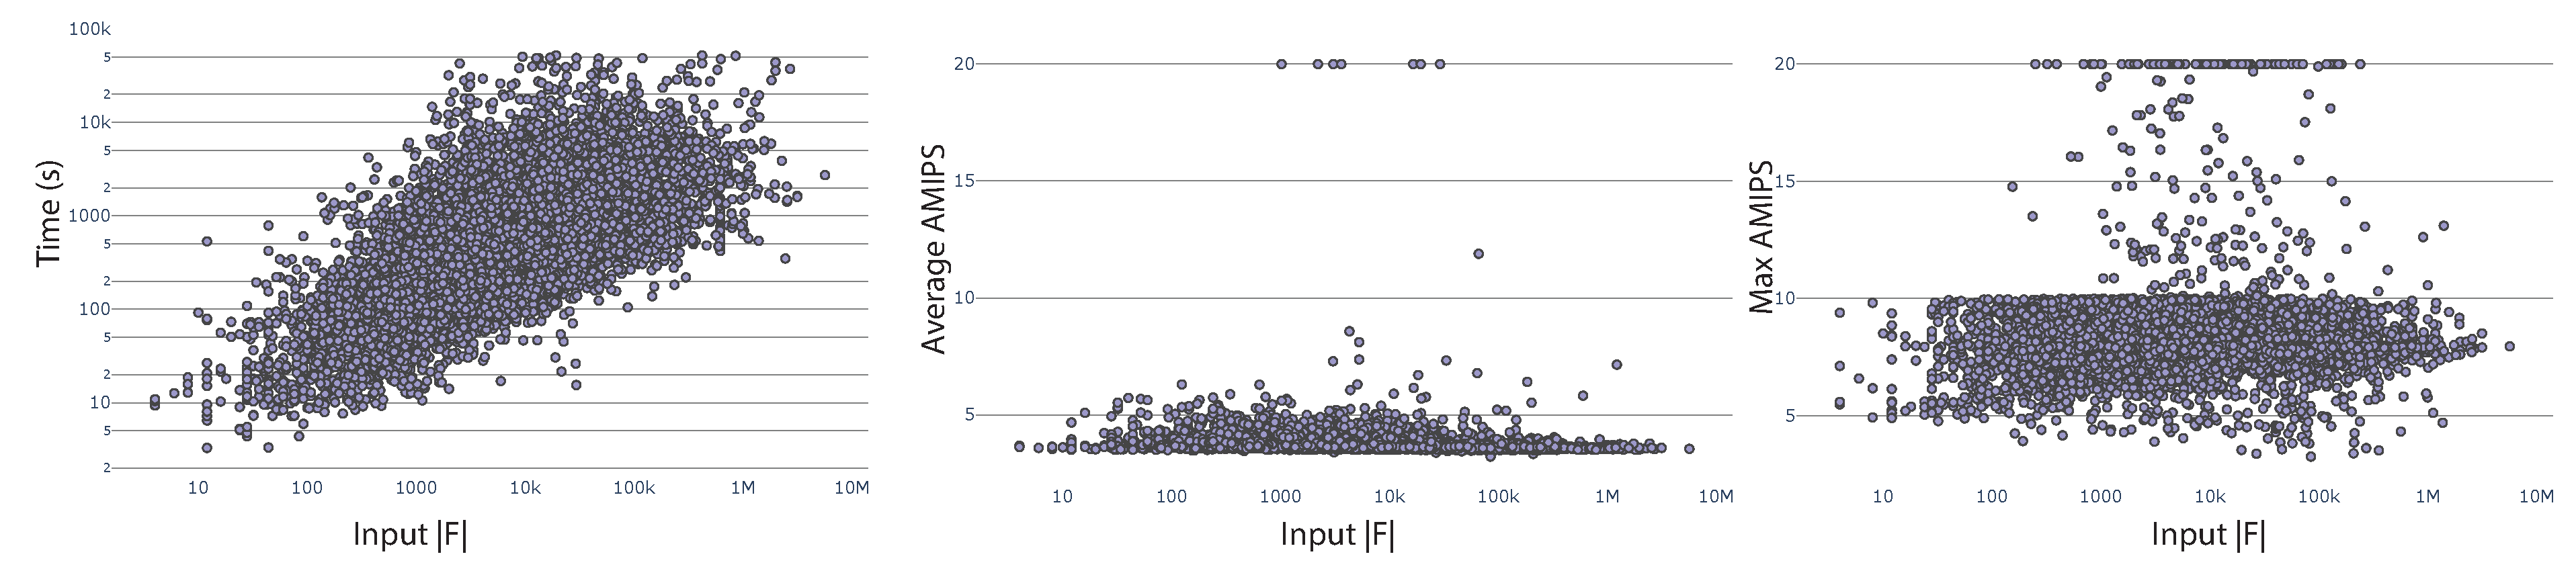
\includegraphics[width=\linewidth]{wmtk-tex/figs/tet3d-stats.pdf}
    \caption{{Timing, max and average AMIPS energy (capped at 20) for maximum 25 iterations of tetrahedral meshing. Most models finish withing 20 minutes with only a few taking up to a day. Even by limiting the iterations to 25, most models reach an average AMIPS energy lower than 10, with optimal value at 3.}}
    \label{fig:3d-datasaet}
\end{figure}

\section{Remarks}

This paper introduces a new declarative specification for mesh algorithms to allow an easier implementation, while at the same time obtaining competitive performances and exploiting parallel hardware. 

Using this specification, we implement {five} popular mesh editing algorithms covering mesh generation and optimization on surfaces and volumes, which can be easily adapted for other use cases: we demonstrated that integrating an envelope check {requires} only a few lines of code.

The library we implemented supports shared memory parallelism, which leads to a good scaling on the machines we tested it on. We believe an exciting venue for future work would be the implementation of a library {for} our specification targeting  MPI to distribute the computation over an HPC cluster. Having access to such a library would allow our five mesh editing applications to run on a distributed environment with minimal or no changes.


%\ZJ{An important limitation (need a positive spin) is that some operations depend on ordering to have optimal performance, and parallelism cannot guarantee that. Like QSLIM, even edge splitting.}

\bibliographystyle{ACM-Reference-Format}
\bibliography{99-bib}
% \appendix
% \input{10_appendix}

\end{document}
